%Carattere dimensione 12
\documentclass[12pt]{report}

%Margini e interlinea
\usepackage[top=2.5cm, bottom=2.5cm, left=4cm, right=2.5cm, centering]{geometry}
\linespread{1.5}

%Librerie utili
\usepackage[english]{babel}
\usepackage[utf8]{inputenc}
\usepackage{scrlayer-scrpage}
\ifoot[]{}
\cfoot[]{}
\ofoot[\pagemark]{\pagemark}
\pagestyle{scrplain}
\usepackage{mathptmx} % font times new roman (simile)
\usepackage{graphicx}
\usepackage{csquotes} % for block quotations
\usepackage{titlesec} % per la formattazione dei titoli delle sezioni, capitoli etc.
\usepackage{float} % per il posizionamento di immagini
\usepackage{titlesec} % per i titoli
\usepackage{listings} % per il codice di programmazione
\renewcommand{\lstlistingname}{Code}% Listing -> Codice
\usepackage{xcolor}  % stile del codice

\definecolor{mygreen}{rgb}{0,0.6,0}
\definecolor{mygray}{rgb}{0.5,0.5,0.5}
\definecolor{mymauve}{rgb}{0.58,0,0.82}
\definecolor{darkgray}{rgb}{.4,.4,.4}
\definecolor{navy}{HTML}{000080}
\definecolor{purple}{rgb}{0.65, 0.12, 0.82}
\definecolor{codepurple}{rgb}{0.58,0,0.82}
\definecolor{backcolour}{rgb}{0.95,0.95,0.92}

%Customize a bit the look
\lstset{ %
belowcaptionskip=0.5em,
backgroundcolor=\color{backcolour}, % choose the background color; you must add \usepackage{color} or \usepackage{xcolor}
basicstyle=\footnotesize, % the size of the fonts that are used for the code
breakatwhitespace=false, % sets if automatic breaks should only happen at whitespace
breaklines=true, % sets automatic line breaking
captionpos=b, % sets the caption-position to bottom
commentstyle=\color{mygreen}, % comment style
deletekeywords={...}, % if you want to delete keywords from the given language
escapeinside={\%*}{*)}, % if you want to add LaTeX within your code
extendedchars=true, % lets you use non-ASCII characters; for 8-bits encodings only, does not work with UTF-8
frame=single, % adds a frame around the code
keepspaces=true, % keeps spaces in text, useful for keeping indentation of code (possibly needs columns=flexible)
keywordstyle=\color{codepurple}, % keyword style
% language=Octave, % the language of the code
morekeywords={*,...}, % if you want to add more keywords to the set
numbers=left, % where to put the line-numbers; possible values are (none, left, right)
numbersep=5pt, % how far the line-numbers are from the code
numberstyle=\tiny\color{mygray}, % the style that is used for the line-numbers
rulecolor=\color{black}, % if not set, the frame-color may be changed on line-breaks within not-black text (e.g. comments (green here))
showspaces=false, % show spaces everywhere adding particular underscores; it overrides 'showstringspaces'
showstringspaces=false, % underline spaces within strings only
showtabs=false, % show tabs within strings adding particular underscores
stepnumber=1, % the step between two line-numbers. If it's 1, each line will be numbered
stringstyle=\color{mymauve}, % string literal style
tabsize=2, % sets default tabsize to 2 spaces
title=\lstname % show the filename of files included with \lstinputlisting; also try caption instead of title
}
%END of listing package%
 
%define Javascript language
\lstdefinelanguage{JavaScript}{
keywords={typeof, new, true, false, catch, function, return, null, catch, switch, var, if, in, while, do, else, case, break, uint256, address, uint, string, bool, let, const, CustomEvent},
keywordstyle=\color{blue}\bfseries,
ndkeywords={class, export, extends, define, super, boolean, throw, implements, import, this, constructor, pragma, contract, modifier, struct, mapping,},
ndkeywordstyle=\color{navy}\bfseries,
identifierstyle=\color{black},
sensitive=false,
comment=[l]{//},
morecomment=[s]{/*}{*/},
commentstyle=\color{mygreen}\ttfamily,
stringstyle=\color{red}\ttfamily,
morestring=[b]',
morestring=[b]"
}

\lstdefinelanguage{HTML5}{
        language=html,
        sensitive=true, 
        alsoletter={<>=-},
        otherkeywords={
        % HTML tags
        <html>, <head>, <title>, </title>, <meta, />, </head>, <body>,
        <canvas, \/canvas>, <script>, </script>, </body>, </html>, <!, html>, <style>, </style>, <query-ui>, </query-ui>, <query-text,  </query-text>, <result-media, </result-media>, <video-editor-app>, </video-editor-app>, <video-preview, </video-preview>, <track-editor, </track-editor>, <video-editor>, </video-editor>
        },  
        ndkeywords={
        % General
        =,
        % HTML attributes
        charset=, id=, width=, height=,\/.dictionaries=,\/placeholderText=,.answerSet=,
        % CSS properties
        border:, transform:, -moz-transform:, transition-duration:, transition-property:, transition-timing-function:
        },  
        morecomment=[s]{<!--}{-->},
        tag=[s]
}
 
\lstset{
language=JavaScript,
extendedchars=true,
basicstyle=\footnotesize\ttfamily,
showstringspaces=false,
showspaces=false,
numbers=left,
numberstyle=\footnotesize,
numbersep=9pt,
tabsize=2,
breaklines=true,
showtabs=false,
captionpos=b
}

\titleformat{\chapter}[block]
  {\normalfont\LARGE\bfseries}{\thechapter.}{0.5em}{\LARGE}
\titlespacing*{\chapter}{0pt}{-20pt}{25pt}

\usepackage{csquotes}
\usepackage[backend=biber, sorting=nty, ]{biblatex}
\appto{\bibsetup}{\raggedright}
\addbibresource{bibliography.bib}

\begin{document}

\begin{titlepage}
\begin{figure}
    \centering
\includegraphics{logo}
\end{figure}

\begin{center}
    {\LARGE{ Corso di Laurea in Informatica Umanistica }}\\
    \vspace{2cm}
    {\Large { TESI DI LAUREA }}\\
    \vspace{2cm}
    {\Large { Remix Culture:
  development of a component based multimedia editing platform }}
\end{center}

\vspace{2cm}

\begin{minipage}[t]{0.47\textwidth}
	{\large{\bf Relatore:\\ Chiar.ma Prof.ssa Maria Simi\\}}
	{\large{\bf \\Correlatore:\\ Chiar.mo Prof. Vincenzo Gervasi}}
\end{minipage}\hfill\begin{minipage}[t]{0.47\textwidth}\raggedleft
	{\large{\bf Candidato: \\ Lukasz Szczygiel\\ }}
\end{minipage}

\vspace{20mm}

\centering{\large{\bf ANNO ACCADEMICO 2020/2021 }}
\end{titlepage}

\tableofcontents
\thispagestyle{empty}

\listoffigures

\thispagestyle{empty}
\clearpage
\setcounter{page}{1}
\addtocontents{toc}{\protect\thispagestyle{empty}}
\addcontentsline{toc}{chapter}{Introduction}
\chapter*{Introduction}
\label{ch:introduction}

% --- Introduction start ---

The Remix Culture is a transformative practice that affects a whole spectrum of creative works. In the digital world, thanks to the Internet pervasiveness, everyone can become a content creator by using and arranging existing contents from various sources. This practice – called “remixing” – can radically change the meaning of the original works during the transformative passage from the “old” into the “new”. Nowadays, this is substantially limited by various laws related to the Intellectual Property Rights. On the other hand, whether it is legal or not, this is what commonly happens in the digital environment. People make various forms of remixes, for example, parodies, memes, mash-ups, and other derivative works. The production of these is enabled by software and stimulated by a number of social platforms which offer these new forms of interactivity. On this regard this dissertation also shows the development of a web application that aims to further explore the possibilities of remixing digital contents. More generally, it seems that remixing can also be extrapolated from a number of other disciplines and physical works, thus leading to a thesis which correlates this sort of behaviour to the human nature itself.

This dissertation aims at making an in-depth analysis of the Remix Culture phenomenon. The benefits and the potential new applications together with some factors limiting its expansion will be discussed in detail later on. Moreover, a review of the state of the art and some proposals about alternative solutions to copyright issues such as Open Source and Creative Commons are some of the topics that will be covered in the first chapter.

Subsequently, an overview from the management perspective with considerations about the sustainability of the Open Source organisations and some best practices for project development will be demonstrated in order to connect the theory to the practice.

Finally, a practical example of a web application that enables remixing was made. The project consisted in creating a multimedia editor for audio visual content. Thanks to this solution users are able to explore and choose multiple media types, namely, videos, images, and audio items from a library of elements. These media can then be viewed, arranged between one another, and inserted inside a multi-tracked editor. Analogously to some popular solutions for video-editing, this allows for real-time preview of the combined elements. The peculiarity or the main software value proposition is that this application works directly inside all the modern browsers.
In particular, the development process will be documented alongside with the explanation of the technical choices and the current software tendencies. Interestingly, this last chapter also advocates for remixing due to the adopted architecture based on reusable components with encapsulated functionalities. From the software perspective the component-based approach allows for interoperability thanks to the adoption of a standardised Web Components technology. In turn, this opens the possibility of combining single components just as LEGO blocks or puzzles. Indeed, this sort of new combinations can be made to produce new applications.

The theme of this work is also connected to the “PH-Remix” project. The acronym stands for “Public History Remix” and it involves the creation of a platform with the subsequent ingestion of resources belonging to the “Mediateca-Toscana” regional foundation. This project’s technical solution aims at exploring new ways of content dissemination, discovery, use and re-use which may enhance the value and the public utility of the uploaded resources. Furthermore, an important element of innovation consists in the automatic extraction of short clips from the videos by using Artificial Intelligence algorithms. For instance, at the time of writing, the uploaded content consists mainly of documentaries. Once uploaded to the platform, the algorithms are able to perform the object recognition task. This task returns a set of recognised objects, for example, people, furniture, ships, animals and many more together with the video frames containing the recognised objects. Hence, these video frames or video clips become short thematic extracts of the original media. Ultimately, they can be offered to the users for exploration and arranged inside the multimedia editing component.

To summarise, the PH-Remix main objectives can be framed into the cultural heritage perspective of digitization of audio-visual resources. It is an attempt to enhance content fruition by encouraging innovative ways of user participation and content discovery. PH-Remix is an ongoing project which involves, at the time of writing, the activity of three researchers from three different areas. Namely: archive’s analysis and cataloguing, data extraction and artificial intelligence, user experience and user interfaces.
Although the development of the web-based multimedia editor originated from the requirements of the PH-Remix project, subsequently it was adapted to fit a general-purpose scenario with a solution that can be modified and expanded upon according to the use case. Nevertheless, the project will be considered as a study case across all the chapters of this dissertation.

To review, the dissertation is logically divided into three chapters.
The main theoretical concepts with examples and copyright issues are explained in chapter \ref{ch:ch1_RemixCulture} Remix Culture.
Considerations about project management and Open Source sustainability are discussed in chapter \ref{ch:ch2_ProjectManagement} Project Management and interdisciplinary works.
The application development process with application examples is inserted in chapter \ref{ch:ch3_ProjectDevelopment} Project development.


\clearpage

\chapter{Remix Culture}
\label{ch:ch1_RemixCulture}

% --- Chapter 1 start ---

Remix Culture is the overarching theme of this dissertation. This phenomenon encompasses a large number of domains and aspects of everyday life involving creativity, thus shaping the way these works are being created, shared, used, and reused. Indeed, the fruition and the reuse are the most characterising facets of the Remix concept.

As mentioned in the introduction, Remix Culture is a transformative practice. By taking one or more pieces of existing items – both physical and digital – new works can be created. For instance, the replacement of an audio source within a certain video or more complex arrangements like entire movies made by using other audio-visual elements are both valid examples of transformative practices. These kinds of remixes can radically change the meaning and the cultural perception of the original works.

It appears that the Remix Culture can be seen from two high-level perspectives, the first tied to the digital evolution. Indeed, among the inspirations of the Remix Culture is the Free and Open Source-Software (“FOSS”), an initiative which will be introduced in paragraph \ref{sec:IPR} \emph{Open Source} as a precursor to the Open Source movement. In short, the goals and ideas of these movements are mainly oriented towards encouraging a “free” distribution of software. “Free” is a vague term that will have to be discussed later in more details.

A second perspective is not exclusively tied to the digital evolution, rather it can be seen as a sociocultural concept that affects several aspects of human behaviour. From a broader perspective, the Remix Culture can be thought of as a way the society works and evolves through history. The idea can be explained by using the popular metaphor of “standing on the shoulders of giants” in the sense used and intended by Isaac Newton\footfullcite{bbcNewton}. Therefore, the ability to discover and enhance knowledge – hence progress as humans – can be reached thanks to the contributions of past and present human generations with the knowledge that had been passed to us.

This concept is further sustained by Lev Manovich in his article “Remixing and Remixability”\footfullcite{ManovichRemixability1}. The author argues that:

\begin{displayquote}
    “[...] most human cultures developed by borrowing and reworking forms and styles from other cultures; the resulting “remixes” were to be incorporated into other cultures. Ancient Rome remixed Ancient Greece; Renaissance remixed antiquity; nineteenth century European architecture remixed many historical periods including the Renaissance […]”.
\end{displayquote}

This excerpt suggests a definition of remixability as a common trait of human behaviour as deducted from a historical perspective. This can be generalised to humans as communities\footfullcite{wikiSenseOfCommunity}, as well as individuals. The latter view becomes the core point of author’s subsequent analysis when describing the modern times. The core point of his argumentation is the major novelty introduced by the Internet, that is the unprecedented level of participation of individuals with the relative ease of accessibility. Indeed, related to this aspect, he states that “culture has always been about remixability, but now this remixability is available to all participants of Internet culture”\footfullcite{ManovichRemixability2}. Nowadays, the pervasiveness of Internet connectivity has led to a professionalization of individuals. Thanks to information available on the web combined with software tools that allow to produce new content, the individuals can become active members of the Remix Culture. Finally, acting as creators, members of the public are able to share their work almost instantly, everywhere and at little or no cost. 

As a matter of fact, this reflects the tendency of new social interactions enabled by the Internet. Many of the most popular online platforms, like Youtube, TikTok, Instagram, etc. make extensive use of the Remix Culture. In the next section \ref{sec:RmxExamples} \emph{Examples of Remixes}, some practical examples of remixes from various disciplines and time frames, ranging from texts, music, films to videogames will be presented to better illustrate the whole phenomenon.

Before expanding further in framing Remix Culture, a first glance on common issues can be taken by reflecting upon this rather radical change of paradigm. Hence, the change from an analogic and physical to a digital environment. It could be argued that the national and international laws have not responded adequately to this change of paradigm. According to Lawrence Lessig, who may be considered among the most prominent figures in favour of this argument, states that: 

\begin{displayquote}

“For the first time, the [copyright] law regulates ordinary citizens generally. For the first time, it reaches beyond the professional to control the amateur— to subject the amateur to a control by the law that the law historically reserved to professionals.”\footfullcite{LessigRemixMA1}

\end{displayquote}

This suggests an underlying problem from a legislative perspective, thereby the copyright law. Further evidence will be provided in paragraph \ref{sec:IPR} \emph{Intellectual Property Laws and Reusability}. The overall point is that by analysing the past and current evolution of works of creativity made by “amateurs” i.e., general public, it seems that the law has taken some stringent measures to limit the Remix phenomenon. This is also true for professionals and large businesses. Additionally, some uncoordinated decisions have been made to respond to certain issues with the practical applications of copyright laws. This overall might be considered as an inhibitory factor acting against the Remix Culture ideas and practical applications.

Another interesting point of view related to the concept of Remix Culture is given by the aforementioned Lawrence Lessig, the founder of Creative Commons. In his book “Remix Making Art and Commerce Thrive” he defines Remix Culture as a Read/Write (“RW”) culture as opposed to a Read/Only (“RO”) culture. The author uses an analogy of how popular computer systems work (for example Linux based systems, Windows etc). Basically, users with read and write permission on a file or directory are authorized to read it and make changes. On the contrary, the read only permission allows only for files and directories to be read disabling the ability of making any modifications.

Returning to the cultural context, the latter is the situation where the users or the general public passively consume the content made by someone else. This is frequently the case of professionally made content, backed by expensive tools and potentially complex organisational structures. For example, the TV broadcasts, production of high budget movies and their subsequent distribution on CDs, DVDs, etc. It could be argued that the Read/Only culture lasted until the times of Internet pervasiveness, as it is characterised by a top-down consumption of cultural objects. On the other hand, the Read/Write culture allows for a democratized participation on the creative process. Hence, a democratization of the act of creativity where people participate in the creation and the re-creation of culture.
These arguments represent a paradigm switch. In the Read/Only culture information flows one-way – unidirectionally –, while in the Read/Write culture the information is multi directional or, speaking in terms of networking: peer to peer like\footfullcite{wikiPeerToPeer}.

At this point, it should be clear that the technological progress allowed to minimize the gap between the professionally created content and the works of creativity that can be made without substantial investments or infrastructure. This can be accomplished thanks to software that makes the technical operation of “remixing” relatively easy.

This concept is also exemplified by Lev Manovich in relation to music remixes and music mashups. In his article “Remix and remixability” he states that: “Although precedents of remixing in music can be found earlier, it was the introduction of multi-track mixers that made remixing a standard practice" \footfullcite{ManovichRemixability3}\,\footnote{This specific example is somewhat related to this dissertation’s practical application. Instead of music as exemplified by Lev Manovich any type of media can be put into a multi-track editor to create new remixes.}.

Hence, what really made the Read/Write culture come to life was the 21st century digital revolution. Indeed, there are some relevant differences between the way things could be created, re-used, and shared before the age of Internet. A notable example showing these differences is the invention of the mechanical movable-type printing press, that is an efficient machine for printing texts. The main difference between the printing press and the Internet is that the printed output copies were inferior to the originals in terms of quality. The affordability was also an issue, costs related to printing a copy prevented people to fully benefit of that invention. Another aspect of this problem is that people had little choice regarding the production of copies for themselves. The alternative choices – until the introduction of low-cost home prints – would imply an inferior quality to those coming from the professional printing businesses. Thus, the whole process relied on professionals.
On the other side, the Internet can be seen as the most efficient, low-cost copying and sharing mechanism accessible from everywhere. Furthermore, the sharing process allows for resources to be distributed globally between connected users, and this is a substantial difference from the previous models. Therefore, users do not often need to rely on professionals to make creative works.

These differences can be further explained from an economical perspective as the distinction between rival goods and non-rival goods\footfullcite{wikiRivalry}. In general, most physical goods are rival goods. For example, a sandwich is a rival good, because the act of eating it clearly diminishes its value. A sandwich loses its value while it is being eaten, so to speak. Sharing rival goods implies the that the benefits of use are decreased or eliminated, so sharing a piece of sandwich produces a tangible loss for the owner of the sandwich. Analogously, sharing a printed copy of a book is an example of rivalry because it prevents the original owner from its unlimited consumption.

On the other side the definition of non-rival goods implies that: "[…] one person’s enjoyment of a good does not diminish the ability of other people to enjoy the same good” \footfullcite{KotchenPublicGoods}. Hence, ideas and words tend to be non-rival. Sharing them does not make them worse or less valuable. An exception of a physical good that is non-rival could be a public bench. The bench value is not significantly diminished when used by people (at least, hopefully, if it is being used correctly). From this perspective a large majority of digital goods are non-rival. A relevant example is an e-book, no one ever “bought” an e-book, people buy a license to read e-books on their devices of choice. Namely, the use of copies does not preclude its accessibility from others and is not directly connected to tangible losses. A few exceptions like domain names and so on exist in this category as well.

Expanding upon the non-rivalry definition, in his book “The Success of Open Source"\footfullcite{WeberOs}, Steven Weber argued that some ideas, words, etc. are definable as “anti-rival goods” meaning that they are improved by being shared in a manner similar to the economics idea of the “Network effect”\footfullcite{wikiNetworkEffect}. Some examples could be the case where a social media gets more powerful as more and more people are using it, or an article becomes more valuable as its hyperlink is being shared across the web, etc. In short, the act of sharing increases the benefits for other participants. For this same reason it could be argued that the efforts to combat climate change are non-rival because the benefits of these actions are shared among all the word’s living species, including for example all the nations who refuse to do so. 
This final point of analysis suggests that the Remix Culture could be in fact non-rival. This argument could be rephrased as a direct question, “are the works of creativity produced as a result of remixing beneficial for the general public?”

Unfortunately, the proposed answer is murky, since from a general point of view it would be very hard to answer with a simple “no” or “yes”. It might be argued that it depends on case to case and on the relative contexts where this question is made. Probably, the answer might not always be positive from the perspective of original creators or de facto owners of works whom creations might be used in a way that contradicts their believes, such as propaganda, commercial profits, etc. Nevertheless, the key point worth considering is that as a matter of fact, everything can be remixed and distributed globally.

In this view, a consideration on the \emph{PH-Remix} project case is pertinent. Among the project’s goals are dissemination, discovery, use and re-use which may enhance the value of created content. From a practical point of view, short clips are extracted from films uploaded to the platform – mainly documentaries at the time of writing – using Artificial Intelligence algorithms. Subsequently, in an idealistic scenario all the clips should become available for remixing i.e., being arranged and combined with other clips to form new audio-visual creations.

However, the tendency of the film industry could be considered sceptical about these ideas or simply not fully aware about the possibilities and new ways of innovating provided by digitisation. Considering the nature of the content initially put on the platform, it could be argued that cultural heritage works and especially documentaries should oblige a moral and ethical motivation of giving back to the communities and not be closed in organisational siloes protected by stringent laws. Indeed, \emph{PH-Remix} for cultural heritage would be a case of non-rivalry because it should be desired to share the messages and stimulate a debate with as many people as possible with as little limits as possible.

Naturally, critiques about the idea of Remix Culture exist\footfullcite{rmxWoRomance}. They will be further discussed in the next paragraph in relation to copyright issues. It could be argued that a relevant part of human progress alongside with some of the most iconic inventions were made thanks to the presence of copyright laws. Nowadays, by taking into consideration that the cost of distributing content is as low or almost nonexistent for digital goods it may still be necessary to reward the creators of intellectual property.

This objectively seems to be true. Remix culture can be enabled by openness and Open Source licenses, but these are not a silver bullet for all projects and creations. A relevant example was once provided during the “Open Cultures” course at King’s College London by Dr John Lavagnino. He argued that J.K. Rowling could probably not have finished the Harry Potter books if she had decided to start publishing them without a license. A source of income is often needed and necessary. On the other hand, the more people who read Harry Potter the better. Generally, as a creator you probably would want to get as many people as possible to watch/be able to consult your creation. In chapter \ref{ch:ch2_ProjectManagement} \emph{Project Management and interdisciplinary works}, arguments advocating for a sustainable economy for content creation – especially for cultural heritage – will be discussed in more detail. 

\section{Examples of Remixes}
\label{sec:RmxExamples}


The practice of modifying both physical and digital items has a long-standing tradition. Remix applies to music, movies, cooking recipes, software, and many other disciplines. After introducing the Remix Culture mainly from a theoretical point of view, it is useful to make some practical examples to better understand the overall concept. For this reason, a selected list of examples from different domains – although mainly focused on the modern age time frame – is presented in this section.

An in-depth study of the creative processes and the way content is being re-used was done by Kirby Ferguson in his four-part video series titled “Everything is a Remix”\footfullcite{everythingIsARemix}. Indeed, he states that the acts of copying, transforming, and combining are the basic elements applicable at any level of creativity. Hence, the following assertion: “creativity is not magic, it happens by applying ordinary tools of thought to existing materials”\footfullcite{everythingIsARemix3}.

Music mashups are one of the most common examples of such transformations. Specifically, hip hop music was one of the first musical forms to incorporate samplings in the recordings\footfullcite{wikiMashup}. Thereby, the results are creative works which typically incorporate fragments of other songs. These fragments are generally re-arranged, thus transformed to produce new sounds and songs. Indeed, in most cases mashups are legal by considering them under the various boundaries of “fair use” law doctrine. These boundaries are usually fuzzy although the tendency of re-using pieces of other songs is very popular among many artists.

One example of a band which crossed boundaries of fair use is Led Zeppelin. They copied significant part of other songs without making fundamental changes. Two documented examples of songs subject to legal claims can be seen on the list below:

\begin{itemize}
\item Led Zeppelin song: “Bring it on home” was a copy of Willie Dixon – “Bring It On Home”\footfullcite{ledZeppelin1}
\item Led Zeppelin – “Stairway to Heaven” most likely copied from the band Spirit with their song “Taurus”\footfullcite{ledZeppelin2}
\end{itemize}

Another discipline which makes extensive use of Remix is the cinema industry. Many movies are inspired by the surrounding works of culture. Nowadays, a common technique consists in transforming the “old” into the “new”. That means taking or re-creating already existing materials from literature, actual events, etc. and producing movies for the current generations. Even existing movies are often a base for new cinema adaptations and frequent prequels and sequels.

One important example of remixing in the film industry are the Disney movies. The Walt Disney Company made extensive use of works from the public domain. Some examples from their repertoire of animated films history are listed below:

\begin{itemize}
\item The Little Mermaid is based on the “The Little Mermaid” fairy tale written by Hans Christian Andersen.
\item Alice in Wonderland is based on the novel “Alice's Adventures in Wonderland” and its sequel, “Through the Looking-Glass” both authored by Lewis Carroll.
\item Aladdin is based on the folk tale “Aladdin from the Arabian Nights” originated from the Middle Eastern culture and later interpreted by Antoine Galland.
\item Mulan is based on the traditional Chinese story of “Hua Mulan”, a legendary folk heroine. 
\end{itemize}

Once transformed into animated movies, Disney likewise any other film producer, were entitled to a period of exclusivity on their productions thanks to copyright. Then after a certain period their work is supposed to enter the public domain to be freely used and built upon. This case was regulated by the American legislation in the Copyright Act of 1976\footfullcite{wikiUSCopyrigh1976} which established the duration of copyright for the life of the author plus 50 years, or 75 years for a work of corporate authorship.

Interestingly, some companies and prominently Disney lobbied to have their terms of copyright extended\footfullcite{wikiUSCopyrighExtensionAct} with the Copyright Term Extension Act, also known as “Mickey Mouse Protection Act”. The company decided to prevent others from copying its works. Therefore, standing to the current copyright terms, Mickey Mouse, which firstly appeared in 1928, will enter the public domain starting from 1st January 2024\footfullcite{mickeyMouse}. It could be argued that by trying to foresee into the future, Disney will attempt to prevent it from happening by using other laws including trademark protection and using precedents in their favour from other court verdicts.

Returning to the practical cases, the film industry is a rich source of similar examples. For instance, an in-depth analysis of the Star Wars series results in finding multiple references and inspirations from historical events, fiction literature, etc. as well as some copied elements from other film productions. It could be argued that without the influence of past creations Start Wars would not have been created.

The digital evolution alongside with the birth of software for video-editing allowed for a more accessible and complex remixing of new content outside of the professional world. Fan-made trailers, remixes, memes that spread virally are all consequences of the ease of use enabled by a mix of modern technology combined with user’s creativity.

Certainly, a long list of important examples could follow. For example, Machinima\footfullcite{machinima} productions, videos generated from video games graphic engines are a relevant contribution to re-use.
The core point is that the strength of these creations is also traceable to the communities of users that participate in the creative process and the consumption. Indeed, there are several examples of Remixes as community efforts.

Perhaps the most well-known and successful community effort is Wikipedia. Wikipedia’s main power is a huge community of active volunteers thanks to which it was able to succeed.

Other projects like Free Beer\footfullcite{freeBeer} and OpenCola\footfullcite{openCola} are examples of remixing in the physical world. They respectively consist in creating and improving recipes for beer and (coca) cola and encouraging their production by adopting a permissive license to the recipes.
In reality, the latter example is connected to the Open Source community as an attempt to replicate the concepts of free sharing and contributing into the physical world which was already a common practice in the software world. 

Naturally, Remix could be viewed as a form of art. Like the latter it is also subject to personal interpretation because, among its goals, is the creation of spaces for debate. Obviously, they often might be a source of tensions and critiques, as the example below.


\begin{figure}[H]
\centering
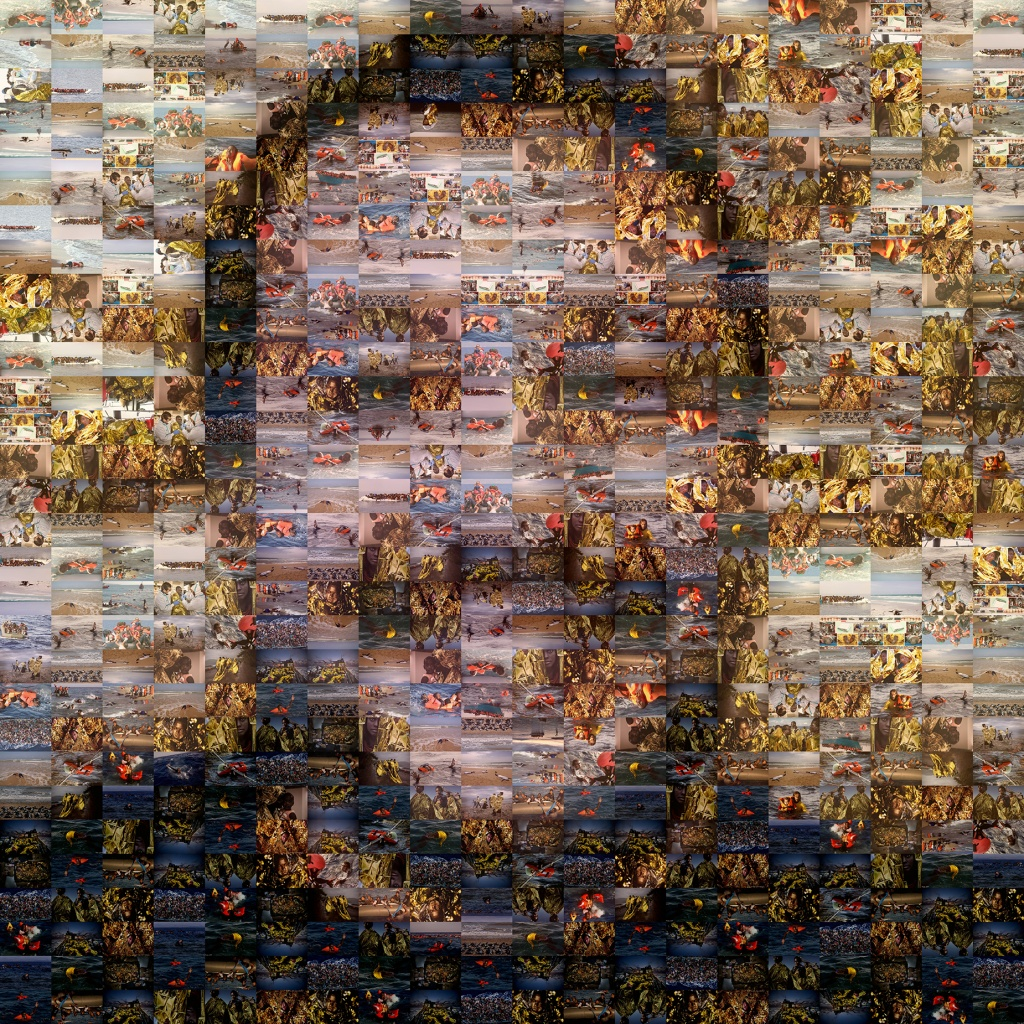
\includegraphics[width=0.6\textwidth]{images/arteAcquaSalvini.jpg}
\caption{"Arte dell'acqua" by students of Russoli High School (Pisa)}
\label{fig:arteAcqua}
\end{figure}

Figure \ref{fig:arteAcqua} "Arte dell'acqua"\footfullcite{arteDellAcqua} is a collage of approximately 400 photos of migrants which depict some tragedies happening at sea while trying to reach the coast. Together the pictures form the face of an Italian politician, Matteo Salvini. He is known for his ideological line against illegal immigration as he advocates for stronger actions and policies to enforce its prevention. Indeed, these forms of remixes can inevitably create controversies. Nevertheless, art encourages reflection and debate and above all it is an expression of free speech.

Lastly, copying is not necessarily equivalent to plagiarism. For instance, this whole dissertation could be seen as a remix. Originated by combining and arranging a set of factual sources with quotations alongside with the author’s academical background, personal experiences, and cultural bias to produce something new. 
While this last example of remix is perfectly legal – if it complies with some rules about academical quotations, etc. – and thus cannot be considered as a plagiarism, the same cannot be said about other contexts and media types.


\section{Intellectual Property Laws and Reusability}
\label{sec:IPR}

Understanding the concepts related to intellectual property (“IP”) and how they are regulated, is fundamental in order to acquire a complete picture of the Remix Culture.

Naturally, the activity of Remix is deeply interconnected with a multitude of laws. It is fair to debunk upfront that an extensive analysis of the topics presented in this section is beyond the scope of this work.  These are complex topics where legal terms involve the use of legal technicalities which differ from country to country. However, understanding the fundamentals of concepts like copyright and licensing is fundamental to explain and to illustrate some frequent problems occurring when adopting the Remix Culture.

As introduced in the previous paragraph, the re-use of content can be substantially limited and potentially discouraged because of the legal bounds applicable to a multitude of physical and digital goods. These legal bounds are typically expressed in form of author’s rights – or copyright, as these terms are used interchangeably in this dissertation – and can be contained in licences applicable to different kinds of works. In short, by creating new works authors are automatically entitled to exclusive rights on them and, as long as a permissive license is not applied, these works cannot be freely reused by others.

In reality, this might often work as a chilling effect, that is, “a discouraging or deterring effect, especially one resulting from a restrictive law or regulation” \footfullcite{collinsChillingEffect}. Furthermore, this effect can also be attributed to the quantity and the complexity of regulations affecting the specific items that might be of interest for re-use. A relevant argument in favour of this assertion comes from a phenomenon called proliferation of licenses\footfullcite{wikiLicenseProliferation}. This is originated from the creation of a large number of similar agreements that might require some domain specific knowledge for their interpretation. Additionally, licenses – whose main goal is to clearly explain the rights and limitations applied to a specific object – are often incompatible between each other, even if they are similar in their permissiveness or strictness.

The subsequent analysis will be focused on illustrating an overview and developing an understanding of the legislative implications of some legal terms that are relevant for the Remix Culture.

Firstly, “Intellectual Property Rights” (“IPR”) is an umbrella term for a category of rights which regulate intangible creations of the human intellect\footfullcite{forbesIPR}.

\begin{displayquote}
“The main purpose of intellectual property law is to encourage the creation of a wide variety of intellectual goods. To achieve this, the law gives people and businesses property rights to the information and intellectual goods they create, usually for a limited period of time.”\footfullcite{IPRightUses}
\end{displayquote}

As seen in the above explanation, the reason for restricting the IPR duration to a limited period of time is mainly motivated by the goal of encouraging further creations. Hence, during the time of “exclusiveness”, authors can earn profit which in turn acts as an economic incentive for creation in the first place.

Secondly, speaking purely in terms of IPR might be considered as an overgeneralization. Richard M. Stallman argues that including different sets of laws under the IPR term is misleading\footfullcite{IPRGNU}. Nevertheless, the subject’s literature about IPR commonly includes a number of typologies of intellectual property belonging to different branches of law. Namely, rights, patents, copyright, industrial design rights, trademarks, registered designs, trade secrets and so on, also depending on the jurisdiction.

As introduced in the previous paragraph, Remix Culture could potentially be influenced by all of these laws. By taking into consideration the most common use cases a subset of IPR typologies can be taken for a deeper analysis. Specifically:

\begin{itemize}
\item Patents
\item Trademarks
\item Copyrights 
\end{itemize}

Patents are used for protecting inventions. Namely, creativity works that are new, not trivial (for experts in the subject/domain) and are useful, thus capable of being used in some kind of industry. Patents give their owners the right to prevent others from making, using, selling an invention without an explicit permission. For example, scientific or mathematical discoveries cannot be patented, as well as a literary, dramatic, musical, or artistic work and many others. On the other side new plant varieties, medicines, machines, innovative solutions to technological problems are generally valid targets for patents.
An ongoing debate regards the creation of software. The European legislation regulated by the European Patent Convention explicitly excludes the possibility of patenting “computer programs” as stated in Article 52 “Patentable inventions"\footfullcite{EPC}. Still, it is subject to interpretation by courts. Vice versa the American legislation tend to allow software patents.

Certainly, from the point of view of the Remix Culture, software patents could have long-term negative effects. Namely, as stated by the Free Software Foundation Europe, “they specifically inhibit the development of useful software by blocking compatibility and interoperability"\footfullcite{fsfe}.

Secondly, trademarks are some sort of signs that distinguish a company or a service from another. They are also frequently used for marketing purposes like branding, product recognition, etc. Logotypes are a classical example of a trademark. For instance, the Nike “swoosh”, the Apple “bitten apple” and McDonalds “golden arches” are among the popular examples of trademarks.

Finally, copyrights regulate that works cannot be copied without the explicit owner’s permission. This applies to any medium. For example, nobody can make a movie based on a book without obtaining the permission of the owner of the book copyright. Copyright can protect literary works, including novels, instruction manuals, computer programs, song lyrics, newspaper articles, and some types of databases. Perhaps the most important characteristic of copyright is that it does not have to be applied for. Everyone gets it even if not aware of it.

These three are just some selected examples that creators should be aware of when doing remixes. Interestingly, it seems that the just introduced concepts are similar between the physical word and the digital world. Therefore, it could be argued that they are a straightforward translation of legislative terms originated from the history rather than new concepts adapted for the 21st century. This can be explained by considering that the technological progress happened very fast and especially the Internet was an abrupt revolution. In his article “The fight to keep ideas open to all” James Boyle, professor of Law at Duke University, analyses the current restrictions of IPR in a digital environment. He also states that:

\begin{displayquote}
“The internet has dramatically lowered the cost of copying, including illicit copying. When the web was first weaved in the 1990s, intellectual-property owners found their property had, involuntarily, been turned into a common. Strong new copyright rules and draconian enforcement seemed to be necessary to tame the rebellious digital commoners and reclaim the level of control that had existed in an analogue world.”\footfullcite{economyst}
\end{displayquote}

As seen in the above quotation, there are aspects that may justify some actions and fears of the copyright holders. In the recent years, policymakers, faced by arguments and lobbying, decided to adopt, and extend a copyright model which currently may seem as more and more unfit for the technological progress.

Nowadays, this led to a growing quantity of issues. In the same article James Boyle affirms that our smartphones are covered by between 5,000 to 15,000 patents and up to 250,000 if considering all the related patents. The general idea of scholars and professionals advocating for a more liberal approach to digital right is that intellectual property in the actual form blocks innovation and can be harmful for the society.

An example, relevant especially at the time of writing, might regard life-saving creations like vaccines\footfullcite{CCcovid19}. As finally stated by Boyle: “In medicine, rafts of patents obstruct research into treatments such as a malaria vaccine; the costs of just identifying the relevant patents is [sic] prohibitive. Such a system is great for patent lawyers, whom I train. It is unlikely to be good for society as a whole.”\footfullcite{economyst}\,\footfullcite{AcadTimesMalaria}

Returning to the digital objects, the copyright laws evolved in terms of their enforcement. Indeed, they can also be efficiently prosecuted – although sometimes wrongly, by using technology. A relevant example is the YouTube Content ID software\footfullcite{GoogleYTID} which automatically checks for the presence of copyrighted materials. This happens when users upload their media to the YouTube platform.

\begin{displayquote}
“The software establishes a link between an existing work and an uploaded work such as a remix. If the content matches, the video may be automatically blocked, or the sound muted, and the user is automatically informed by e-mail that the material has been disabled”.\footfullcite{wipo2015}
\end{displayquote}

From this perspective, it might be deducted that a potentially dangerous direction would consist in maintaining the current state of IPR and enforcing it through the use of technology. This could be especially harmful for the Remix Culture phenomenon.

\subsection{Derivative Works and Fair Use}

As introduced in the previous section, the Remix Culture often faces problems regarding the legal bounds. Namely, the Intellectual Property Rights. On the other hand, the law also imposes rules and exceptions under which legal works can be created. Specifically, the concepts of derivative works and fair use are key for limiting the application extent of IPR.
In the practical applications of remixes, it seems that a common source of problems derives from how contents coming from a variety of sources are used and distributed for the creation of new works. Indeed, this discourse could be framed into the legal perspective by using the term of “derivative work”. By considering the definition from the Merriam Webster legal dictionary, a derivative work is defined as a “a piece of intellectual property that substantially derives from an underlying work”\footfullcite{merriamWebsterDerivativeW}.

From a general perspective, the notion of derivative works seems to be consistent across many national and international legal systems. Albeit the usage of the adverb “substantially” is the key difference leading to different interpretations as explained with further details later in this section. 
For instance, the United States Copyright Act states that, a “derivative work is a work based upon one or more preexisting works […]”\footfullcite{CornellUSCode}. This definition is followed by a list of actions and types of works that make a derivative work as such.
Along these lines, the 2nd article of the International Berne Convention, entitled “Protected Works”, also refers to the derivative works together with the criteria for its protection. 
“Translations, adaptations, arrangements of music and other alterations of a literary or artistic work shall be protected as original works without prejudice to the copyright in the original work”\footfullcite{BerneConvention}.

Nevertheless, it seems that international and national legal systems are not sufficiently precise when defining derivative works. As a matter of fact, it is very complex to establish which copyrighted materials and above all to what extent, can be used in a new creation without violating the author’s laws. In this view the Remix Culture could be defined as a culture or society where the production of derivative works is allowed and therefore encouraged. Overall, at the time of writing it appears that this is not the case.

One last concept regards the fair use. Specifically, it is the part of the copyright law that allows for free speech (at least in the context of the American First Amendment). Thanks to fair use small amounts of copyrighted materials can be used to make an argument without asking the copyright holder for permission. As stated in the section \ref{sec:RmxExamples} \emph{Remix examples}, this dissertation could be thought of as remix. This is the case of text; the same degree of freedom is illegal in, for example, the filmmaking industry. Limitations like those valid for many academic books – stating that around 15\% of the total pages can be photocopied – do not exist for other digital objects. This prompts an open question about the possibility of imposing similar limitations to digital objects. This would significantly reduce ambiguities and issues with the interpretation, but from a practical point of view may be unfeasible. According to the European law the concept of fair use is fuzzy and does not provide clear guidelines for those who would want to remix content.

An important contribution expanding upon the problems of copyright is RIP: A Remix Manifesto. It is a documentary about “the changing concept of copyright”, and its main point is to illustrate that copyright is not under control\footfullcite{RIP}. Therefore, advocating for the so called copyleft as opposed to copyright. As a matter of fact, even with tools like derivative work protection and fair use, it is not enough to truly incentivize creativity and producing a rich public domain open to all.

Looking at the state of the art, the introduction of the recent European copyright directive (the directive on copyright and related rights in the Digital Single Market, in short, DSM directive) 2019/790 EU\footfullcite{EU2019/790} was supposed to give clarity by regulating many of the edge cases by adapting the IPR to the digital environment.
At the time of writing, it might still be too soon to understand the implications it will have for the digital market and the prosperity of the Remix Culture. Moreover, some studies argue that the DSM will not provide significant improvements for the digital age. “For sure, legal and practical consequences cannot be properly evaluated at this stage, as it is necessary to wait for the implementation of the Directive by all Member States”\footfullcite{springerEU2019}. The directive provides some limited options in terms of specific content like those belonging to the cultural heritage. For example, the Art. 6. concerns the acts of reproduction of some cultural heritage institutions’ works, but it is only valid for preservation purposes.

As stated before, it is difficult to understand the boundaries until the first interpretations are given in courts. The recent history shows that the interpretation of the directives about copyright can give some practical hints for the interpretative direction that will be taken. There are multiple examples of existing cases that show what is legal and what tend not to be. Some interesting examples are the “Tom Cabinet case” (regarding the reselling of second-hand e-books)\footfullcite{EULEXTomCabinet} and “Nils Svensson and Others v Retriever Sverige AB” (case on linking/hypertext that redirect Internet users to protected works available on other websites without the authorisation of the copyright holder)\footfullcite{EULEXSvensson}.

Until this situation is not fully transparent, a valid solution to reduce the risks may come from the use of Open Source and permissive licenses. These will be discussed in the subsequent two sections.

\section{Open Source}
\label{sec:OS}

Generally, the topic of “Open Source” tends to be well recognised within the discipline of computer science and similar, arguably less within other fields. This is mainly due to the fact that it was originated in the context of software development, and thus among computer programmers. However, it is relevant for the Remix Culture not only due to the pure software implications, but also from an organisational and legislative point of view. Thanks to the Open Source and the Creative Commons licensing a more transparent, and accessible picture of remixing will be introduced.

First of all, Open Source does not mean “free” as this can be a common misconception due to its cultural meaning. A brief excursus into the Open Source history ought to be made to understand and explain the terminology used in the subject’s literature.
Historically, around the 1970s with the popularization of personal computers – mainly due to their economic affordability – many programmers started contributing and sharing for “free” their source code with the programming community. However, after some years the progress of the computer industry and the related business models showed a tendency of making proprietary systems, that is closed source programs and systems.
To contrast this phenomenon, ways of regulating the freedom of the source code were necessary for legal reasons. From a practical point of view, a few developers would be interested in contributing to a system that eventually could become proprietary, hence loosing all their voluntary efforts.

For the record, the US Copyright Act was introduced in 1976 with the subsequent result of encouraging the development of proprietary software.
For this reason, Richard Stallman founded the Free Software Foundation. In 1983 he defined the term “free” as a combination of four essential freedoms that must exist in order to define software as free\footfullcite{GNUFreeSoftware}.

\begin{itemize}
\item Freedom 0: The freedom to run the program as you wish, for any purpose.
\item Freedom 1: The freedom to study how the program works and change it so it does your computing as you wish.
\item Freedom 2: The freedom to redistribute copies so you can help your neighbour.
\item Freedom 3: The freedom to distribute copies of your modified versions to others.
\end{itemize}

Subsequently another shift in terminology was deemed as necessary. According to Bruce Perens, the founder of the Open Source Initiative, on a business level the Free Software Definition was not well received. Apparently, managers and executives were not keen to investing on projects with the world “free” incorporated.
“Free” is a difficult term, particularly in the anglophone languages, because it could mean “with no price” or “with no conditions”.
“The Free Software Definition defines the “free” in free software as being about liberty, not price: it is consistent with the principles of free software to sell copies”\footfullcite{Pomerantz_Peek_2016}.

Therefore, speaking in terms of the aforementioned four freedoms, it would mean restricting any of those. Overall, the term “free” is historically overcharged with different connotations and this made the term “open” more adequate as a technical term. Therefore, the shift from the term “free” to “open” began. Nevertheless, in this context the core meaning of both of these terms indicates that the software is the only thing that is gratis. “Just as with proprietary software, there is a “total cost of ownership” of free and Open Source software, which includes such costs as development, customization, maintenance, hardware, support, and many others”\footfullcite{Pomerantz_Peek_2016}.

This is an important clarification as it specifies the contextualized nomenclature of these terms. Particularly, the issue with the term “free” is that it does not clearly reflect the costs connected to the effective software fruition. As a matter of fact, software is complex, thus obtaining it without cost could be thought of as a mere beginning.

For example, there are a lot of digital services that are not open. Services offered by companies like Amazon, Facebook, Google, etc. are mostly not open. They are based on terms of use which limit how these platforms can be used. Arguably, they are not even gratis as users pay by giving the ownership control on a set of their personal data.
On the other hand, Wikipedia is definitely a success story of the Open Source. It is entirely open in terms of systems and content. It allows for reuse of its structure and data. Everyone can host their own Wikipedia page and modify it without restrictions. As a matter of fact, Wikipedia is based on the MediaWiki platform\footfullcite{mediawiki} which is a Content Management Platform (“CMS”) for open contributions and powers multiple community driven wikis, for example fandoms (“Wikias”) focused on various topics. Since thanks to MediaWiki anyone can copy, paste, install, and develop their own solution based on the platform, a straightforward comparison with the Remix Culture can be made. This is an example of an ideal scenario where the Remix Culture can be applied almost without any constrains.

Wikipedia is not the only case of a successful Open Source project. Returning to the aforementioned number of patents in smartphones, described in \ref{sec:IPR} \emph{Intellectual Property Laws and Reusability}, it is safe to affirm that they would not work without the Open Source. One relevant example is the Android operating system which itself is based on Linux. The promiscuity of proprietary solutions and Open Source is possible thanks to the software modularity. A principle whose practical demonstration is discussed in further detail in chapter \ref{ch:ch3_ProjectDevelopment} \emph{Project development: web application for multimedia editing}. Some of the most used commercial systems depend on Open Source components. The Open Source model can also be considered as a valid approach from the managerial perspective. This will be further explained in the next chapter.

As far as this dissertation’s project is concerned, the rationale behind making an Open Source multimedia editor could be that there are not many existing in-browser solutions that allows for video-editing. Systems like YouTube, Vimeo, Adobe Spark and similar are closed source and cannot be reused for the purpose of building personal solutions. Although the solutions proposed for this dissertation practical application are related to the front-end architecture, a more complex back-end solution can be connected for creating custom projects. Thanks to the components approach, a contribution to Open Source is made by making the software available to the community.

\section{Creative Commons}
\label{sec:CC}

Nowadays the usage of licensing has largely widespread thanks to the Internet. A license or copyright license “is a contract which grants certain rights to use a work or other protected materials”\footfullcite{sarah_dominique_orlandi}.

Back in the day, the aforementioned US Copyright Act from 1976, was perceived as too restrictive by the Open Source supporters\footfullcite{Pomerantz_Peek_2016}. This led to a creation of a non-profit organization called Creative Commons (“CC”). Founded in 2001 by Lawrence Lessig, it defines a set of licenses providing alternatives to the traditional copyright. Most importantly these licences allow for creators to specify upfront how and when their work can be used, shared, and remixed by others. As stated in the Creative Commons website, “[the CC] licenses give everyone from individual creators to large institutions a standardized way to grant the public permission to use their creative work under copyright law”\footfullcite{ccLicenses}.
Indeed, the existence of copyright laws is important for Open Source licensing in order to grant usage of something “free of charge” but requiring, for example, that the re-distributing would happen under the same terms. Thus, it enforces rules for something that comes without charging money. Without copyright it would be impossible to do that. Moreover, by defining these agreements using non-legalese, human-readable definitions the CC became a very powerful enabler of openness\footfullcite{Pomerantz_Peek_2016}.

Indeed, the Creative Commons Licenses are based on four rights that can be combined to form a set of licenses. These four clauses are:

\begin{enumerate}
  \item Attribution: All distributions of a work, and derivative works based upon it, must be credited to the creator of the work.
  \item Non-commercial: Derivative works cannot be destined for commercial use.
  \item Share-alike: Derivative work must be licensed under terms identical to those of the original work.
  \item No Derivatives: A work may be redistributed, but only “unchanged and in whole;” no derivative works may be made based on it.
\end{enumerate}

Subsequently the Creative Commons organisation defines six licenses\footfullcite{ccLicenses} starting from the most open to the most restrictive.

The first two license types allow reusers to distribute, remix, adapt, and build upon the material in any medium or format, also allowing for commercial use. The only requirements are that an attribution must be given to the original creator (CC BY license) and the adaptations – thus any modification made to the original work – must be shared on under the same terms (CC BY-SA).

\begin{itemize}
  \item Attribution - Attribution only (CC BY)
    \begin{figure}[H]
    \centering
    
\includegraphics[width=0.3\textwidth]{images/by.png}
    \caption{Attribution CC BY}
    \label{fig:ccBY}
    \end{figure}
    
    \item Attribution - Share alike (CC BY-SA)
    
    \begin{figure}[H]
    \centering
    
\includegraphics[width=0.3\textwidth]{images/by-sa.png}
    \caption{Attribution CC BY-SA}
    \label{fig:ccBYSA}
    \end{figure}
 \end{itemize}
 
The next two license types allow reusers to distribute, remix, adapt, and build upon the material in any medium or format for non-commercial purposes only. Analogously to the first two types a credit must be given to the creator (CC BY-NC) and the adaptations must be shared under the same terms (CC BY-NC-SA).

 \begin{itemize}
    \item Attribution - Non-commercial (CC BY-NC)

    \begin{figure}[H]
    \centering
    
\includegraphics[width=0.3\textwidth]{images/by-nc.png}
    \caption{Attribution CC BY-NC}
    \label{fig:ccBYNC}
    \end{figure}
    
    \item Attribution - Non-commercial - Share alike (CC BY-NC-SA)

    \begin{figure}[H]
    \centering
    
\includegraphics[width=0.3\textwidth]{images/by-nc-sa.png}
    \caption{Attribution CC BY-NC-SA}
    \label{fig:ccBYNCSA}
    \end{figure}
 \end{itemize}
 
The following license differs from the aforementioned types since it forbids the production of derivative works. Thus, adaptations are not allowed, but the work can still be used commercially (as long as credit is given to the author).

\begin{itemize}
    \item Attribution - No derivative works (CC BY-ND)

    \begin{figure}[H]
    \centering
    
\includegraphics[width=0.3\textwidth]{images/by-nd.png}
    \caption{Attribution CC BY-ND}
    \label{fig:ccBYND}
    \end{figure}
\end{itemize}

Similarly to the above CC BY-ND license, the following one works exactly the same, with the exception that it does not allow for the commercial reuse.

\begin{itemize} 

  \item Attribution - Non-commercial - No derivative works (CC BY-NC-ND)

    \begin{figure}[H]
    \centering
    
\includegraphics[width=0.3\textwidth]{images/by-nc-nd.png}
    \caption{Attribution CC BY-NC-ND}
    \label{fig:ccBYNCND}
    \end{figure}

\end{itemize}

Finally, another tool called “Public Domain Dedication” or “CC0” allows for waiving all the related rights and effectively put the work into the worldwide public domain.

    \begin{figure}[H]
    \centering
    
\includegraphics[width=0.3\textwidth]{images/cc-zero.png}
    \caption{Public Domain Dedication}
    \label{fig:cc0}
    \end{figure}

“CC0 allows reusers to distribute, remix, adapt, and build upon the material in any medium or format, with no conditions.”\footfullcite{cc0}

The CC licenses do not contain specific terms about the distribution of source code because they are mainly focused on writings, visual arts, and other creative works. Alternative forms of permissive licensing specifically made for software production also exist. One source containing the range of licenses that are around is: “Various Licenses and Comments About Them”\footfullcite{gnuLicenses} by the Free Software Foundation which provides a list of software licenses with explanations.

By combining the Open Source and Creative Commons the Remix Culture can thrive with new works of creativity which are perfectly legal. An ideal solution would be to propagate the ideas and an understanding of the Creative Commons licenses to encourage their usage among all levels of actors hoping that the openness will create a virtuous cycle that benefits everyone involved.

\clearpage

\chapter{Project management in interdisciplinary projects}
\label{ch:ch2_ProjectManagement}

% --- Chapter 2 start ---

To be continued. 

\section{Interdisciplinary projects and the GLAM sector.}

To be continued. 

\section{State of the art: online video-editing tools}

To be continued. 

\clearpage

\chapter{Project development: web application for \\ multimedia editing}
\label{ch:ch3_ProjectDevelopment}

% --- Chapter 3 start ---

This chapter is meant to illustrate the main thesis about the Remix Culture by combining most of the topics presented in the previous parts into a practical example of project development. The project consists in developing a web application for multimedia editing that can run in every modern browser. Hence, from a general point of view this can be seen as an implementation of a set of features that are common in many offline and online tools for video-editing, as analysed in section \ref{sec:stateOfArt} \emph{State of the art: web video-editing tools}. In more detail, the application main value proposition is to offer the possibility of “remixing” different types of multimedia content, in particular videos, images, and sound media. Thanks to this universally accessible and Open Source technical solution the Remix Culture can come to life and can be experienced by anyone with an internet connection.

More details about the requirements, technical decisions and considerations can be found in the paragraph \ref{sec:SoftwareArchitecture} \emph{Project idea and Front End Software Architecture}. At this point, the main argument is addressed from the perspective of software development. Specifically, the results presented in this this chapter follow a two-pronged objective.

Firstly, the development of an application for remixing multimedia enables users to experience the concepts of the aforementioned Remix Culture by enhancing content discoverability and stimulating user’s creativity. On the other side, content holders, i.e., authors, institutions, etc. can gain in recognition, thus receive added value from this kind of application. Therefore, this can be seen as an attempt to promote the Remix Culture among institutions which may be encouraged by the benefits and decide to upload content on the platform. A particularly suitable target might consist of cultural heritage organisations with their frequent digitalization programmes. These institutions’ digitization strategies often set their priority goals for enhancing user engagement and participation.

A second objective comes from the choices made for the technical architecture. The video-editing tool is open for modifications in terms of software development. By publishing and applying the “MIT” license\footfullcite{mitLicense} to the source code, a contribution to the Open Source is made. Furthermore, by adopting a component driven development with a solution based on Web Components technology – a standard and framework agnostic solution as explained in paragraph \ref{sec:webComponents} \emph{Web Components} – the technical solutions are offered to the community as a library from which to choose from, expand upon, and create brand new projects.

In the next paragraph, \ref{sec:reuseAndMaintainability} \emph{Reusability and maintainability, through abstractions to a component-based approach}, an analysis of the modern software development is presented together with arguments in favour and against the adoption of a component-based approach.

Finally, at the end of this chapter, two examples of application instances will be made: the first example was developed in the context of the “PH-Remix” project. In this case, as mentioned in the introduction, the content belongs to the “Mediateca Toscana”\footfullcite{mediateca} and the development was guided by the requirements expressed in the regional project grant. The project involves several researchers, and the development is still in progress as the project deadline is set to 2022. Therefore, a front-end component (or set of components) was implemented, in anticipation of the back end architecture, while work on the latter is still in progress at the time of writing.
The second application integrates a variety of Open Source materials. It is an example of reusability of the components architecture that can be used for different purposes. The implementation is based on the public Pexels API\footfullcite{pexels} which offers a large number of videos and images. All the content can be used thanks to a permissive license. This solution acts as an aggregator of Open Source licensed materials to create new general purpose productions. It is not connected to any specific target audience. An example could be the discovery of content to be used as commercial advertisement for any kind of industrial product.

\section{Reusability and maintainability, through abstractions to a component-based approach}
\label{sec:reuseAndMaintainability}

Modern software development techniques and tendencies are mainly concerned with the objective of simplifying the development of technical solutions, as well as easing up code reusability and maintainability.

Nowadays, programming – the activity of writing a code – involves the use of a growing number of abstractions as a way of responding to the challenges deriving from the complexity of modern software applications. R.C. Martin in the introduction of Clean Code\footfullcite{CleanCode} affirms that:

\begin{displayquote}

“[…] the level of abstraction of our languages will continue to increase. I also expect that the number of domain-specific languages will continue to grow. This will be a good thing. But it will not eliminate code […]”. 

\end{displayquote}

As the author confutes the “no-code development approach”, he also states that the code will be evolving as an expression of the software specifications. These specifications or requirements need to be translated into a form that is understandable and executable by a machine. Hence, the concept of abstractions will be analysed as one of the guiding principles of software evolution.

Focus will be put on the front-end development ecosystem, as it reflects the majority of work done for this dissertation practical application. Despite this choice, most of the arguments presented apply to the software world in general. The final aim of this paragraph is to provide the rationale behind the choice of Web Components as the technology for project development. As a matter of fact, before introducing Web Components, to fully understand the component-based approach, an introspection into the web development stack ought to be made.

The front-end development is commonly considered as a fast-paced environment among developers\footnote{It is worth noting how this statement can be sustained by real world data. Stack Overflow makes yearly surveys among its community of developers. The Stack Overflow Annual Developer Survey (https://insights.stackoverflow.com/survey/) contains a section called “trending techs” where the rise and decrease in popularity of web development technologies over the years can be analysed in further detail}. In short, the lifecycle of the technologies used for the web application layer is shorter compared to the rest of the software world. Consequently, programmers usually need to make a significant effort in order to stay up-to-date on the recent technological progress. In other words, front-end frameworks and libraries tend to become less maintained, and thus deprecated in a short span of time.

Although the fundamental programming skills required for creating web applications – ranging from simple static websites to complex online platforms – are still based on HTML, CSS, and JavaScript, several solutions were created for more efficient and effective way of reaching programming goals. A relevant example of this evolution is provided by JavaScript frameworks and libraries. It is worth emphasizing that JavaScript started off as a scripting language, generally used for small tasks like adding interactivity to the web pages. As of today, it has become a mature and widely used language both on the front-end and the back-end side (mainly thanks to the development of V8 JavaScript engine used for runtimes environments of Node.js, Deno etc.).

On the front-end side, the progress might be viewed as a development of proprietary and Open Source systems that implement features with the goal of easing up and speeding up the development of web projects. Starting from the jQuery library in 2006, which offered a cross-browser compatible set of features with an API that simplified the most frequent actions like DOM traversal, event handling etc., to the first frameworks (Backbone, Ember, Angular just to name a few) with more sophisticated features like data binding, dependency injection, routing and many more. Another popular, more recent example is the React library.

One of the core innovations of the React library is its design principle of “composition of components”. This principle consists in building “encapsulated components that manage their own state, then compose them to make complex UIs”\footfullcite{reactDesignPrinciple1}. This innovation, as seen in React, reflects the tendency of many other modern front-end frameworks, such as: Vue, Angular, Svelte, etc. They are based on the idea of splitting codebases into small reusable pieces of code, called components. This approach is particularly useful for medium and large software projects as it enables modularization, by splitting software logic into separate modules, thereby encouraging reusability and maintainability. Another benefit of this approach is that the development process can also be better organised between multiple teams working on different features. 

As more and more solutions were introduced into the web development ecosystem, a phenomenon commonly called “proliferation of frameworks”\footfullcite{proliferationFrameworks} became an issue. An issue that might have consequences beyond the vastity of the offer to choose from.
An immediate consequence of using frameworks is the framework-specific way of developing code or components. The developers are required to learn a new framework and dedicate to it in order to gain the benefits that are being offered by those solutions. A flaw of this approach logically follows as the development becomes limited to the specific framework or technology. It seems that more arguments on the downside of using frameworks can be made. The possible common issues involve their lifespan and changes due to new releases that may lead to issues with compatibility between the old and the new versions. Also, the size of the framework codebase, i.e., the functions installed and required by default – often not necessary in every project – can slow down the application performances.
For some projects this might be a viable solution, as for companies currently developing solutions that might benefit from specific features and differences offered by frameworks or for those who can avail of having an internal expertise to justify the usage of a specific framework.

Many of these new features offered by the above tools are connected to the standardization process itself. It seems that the creation of new solutions that gain popularity within the community stimulate the implementation of these features into web standards. Notably, in this context, W3C recommendations standards\footfullcite{w3c} and JavaScript ECMAScript specification \footfullcite{ecma}.Arguments in favour of this thesis can be made. For example, the standard Selectors API specification\footfullcite{w3cSelectors}, offering “querySelector” “querySelectorAll” interfaces for finding elements inside the DOM tree structure, was inspired by the jQuery selectors helper methods\footfullcite{jQuerySelector}. From the perspective of frameworks or libraries adopters the benefits of adopting the libraries over the native standard – which is faster – are inversely proportional to the number of features that exist in the standard. Although nothing prevents developers from adopting jQuery and similar solutions, their adoption may make less and less sense leading to their natural decline.

This prompts the question, if the component approach seems to be a shared direction for developing more complex front-end systems, how to tackle the issues regarding supposedly one of the main features of components, namely the benefit of writing a reusable code while being locked-in into specific technology stacks?

A possible answer might be in the Web Components technology which enforces the property of reuse among applications. In short, having a standardized way of building components would mean greater reusability, configurability, and consistency – avoiding technical lock-ins – for many years to come. As a general rule of thumb, Web Standards, made by W3C and similar, are more reliable than the proprietary Long Time Support (“LTS”) solutions. Web components are a set of Web APIs that allow to create custom, reusable HTML elements with logic and styling encapsulated into their definition. They can tackle the problems of developing interoperable components. By inserting the components within the frameworks, they are expected to work in a plug and play manner thanks to the native APIs compatibility\footfullcite{customElementsEverywhere}.

Nevertheless, Web Components are not to be considered a silver bullet for solving issues presented in this section. Currently, it appears that some problems could also be mitigated by adopting a set of techniques and strategies such as “Micro-Frontends”\footfullcite{microFrontends}. The latter combined with “Webpack Module Federation” seems a particularly promising solution. A detailed analysis is beyond the scope of this dissertation. However, for a better perspective of the current state of art, the idea of Micro-Frontends could be summarized as the application of microservices architecture to the front-end world. As it happens with the back-end, the aim is to decouple the single pieces of an application in a way that they can be developed independently and using different technologies. From a business point of view, this would make sense in large projects and is a promising approach to Agile methodology as small teams could work on developing autonomous features. The key difference between the Web Components approach and the Micro-Frontends is that the development of interoperable components can be done by using different frameworks. A quick example could be a coherent application composed by components made with the Vue, React and Svelte frameworks. Certainly, this leads to complexities. Therefore, the Webpack Module Federation was introduced. This Webpack feature allows a JavaScript application to dynamically load code from another application without compromising security\footfullcite{webpack5}.

In this panorama, the Web Components technology seems like an additional asset to the current way of developing front-end projects. Its aim does not involve replacing the actual front-end frameworks, it should rather be considered as one of the possible ways for adopting a component-based approach on the web. 

Returning to the “PH-Remix” case study, the Web Components were adopted as a front-end technology in line with the project architecture. As a matter of fact, the project architecture is based on a microservice model that allows for a degree of flexibility and enables a parallel development of the back-end infrastructure. Also, from the project development point of view, relying on the standard allows for future developers to modify and enrich the code more easily. Consequently, the necessity of learning new frameworks is absent. This suggests that the features that Web Components offer could solve some of these problems. Indeed, the main promise of making a flexible architecture seemed to be easily solved thanks to this front-end technology of choice. In the next paragraph the main standard’s features will be introduced. 

\section{Web Components}
\label{sec:webComponents}

To reiterate the definition from the last paragraph, Web components are a set of Web APIs that allow to create custom, reusable HTML elements with logic and styling encapsulated into their definition. From a practical point of view, modern browsers can compute Web Components in the form of custom HTML tags that, in turn, can be used and re-used across multiple projects and technology stacks. The described behaviour is equivalent to the one of standard HTML elements as defined in the HTML documentation.

Web Components offer a native platform and a technology agnostic component model for developing a code that runs in browsers. As a matter of fact, this follows the tendency of many modern front-end frameworks, which are based on the idea of splitting codebases into components, as mentioned in this chapter’s introduction. The main difference is the interoperability provided by adopting the solution introduced in this chapter.

Web Components technology can be considered as an umbrella term that encompasses three distinct Web APIs: Custom Elements, Shadow DOM, and HTML Templates. By defining and referring to Web Components as a native technology, the standardization by W3C is intended. The specifications for each of these Web APIs are now incorporated as a living standard\footfullcite{w3cEvergreenStandards}. Each of these specifications will be explored with more detail in the next sections to explain their features and the current limits of this technology. The purpose of these explanations is to provide some basic knowledge about the internal mechanisms and a few points of interest relevant to the subject that might be of interest for readers.

The formal documentations and technical definitions hardly give the developer’s perspective and community feelings about this topic. Therefore, another aspect worth investigating regards the evolution and the adoption of Web Components.

The proposal of Web Components is not new, speaking in terms of software development dynamics. Firstly introduced in 2011 by Alex Russell\footfullcite{webComponentsBeginning}, it went through years of standardization process. The latter might be also viewed as search for consensus between browsers producers, namely the owners of: Safari, Firefox, Chrome – therefore, all the Chromium based browsers – and Microsoft browsers. While the Microsoft browsers consist of Internet Explorer and Microsoft Edge, the former has reached the end of its lifecycle maintaining only the technical support and security updates for its latest version (Internet Explorer 11). The browser does not support the Web Components standard\footfullcite{canIUseComponents}, therefore its implementation and usage require the adoption of polyfills and transpilers.
Generally, transpilers are used to compile the source code written in one language to another. Although in this case their main usage is to transform the code written using some – usually recent – standard into a backward compatible code that can work with the old browsers not supporting that standard. One example of the most popular transpiler is Babel\footfullcite{babel}, which allows developers to use the most recent JavaScript features among all the browsers by translating them into a code compliant with the old language standards.


Returning to the issues of browser compatibility, the deprecation of Internet Explorer and the subsequent evolution of its successor, Microsoft Edge, gave Web Components a boost in terms of compatibility. The main reason can be linked back to the Microsoft Edge passage to the Chromium Open Source project on 8th April 2019\footfullcite{microsoftEdge}. This fundamental change consisted in a passage from the combination of EdgeHTML browser engine and Chakra JavaScript engine to Blink and V8, respectively a browser engine and a JavaScript engine.

This led to a substantial improvement and larger adoption by the community. However, this overview draws attention to the standardization process. As seen, almost ten years were necessary until one of the last major browsers adopted the initial proposal. In the meantime, the standard itself came through a long process of maturation and stabilisation\footnote{An interesting lecture by Jan Miksovsky on how the standardization of HTML slot element may give a better view on the complexities of standardization process: https://component.kitchen/blog/posts/a-history-of-the-html-slot-element}.

The longevity of the process exemplified above might imply and justify the existence of critiques against the Web Components standard. By investigating the most common reasons, it appears that they were mainly concerned with cross-browser discrepancies, partial standard adoption, and frequent API changes. Serhii Kulykov, a developer currently working at Vaadin – a company which uses Web Components with an Open Sourced web application platform – critically reviews in his series of blogs\footfullcite{devToWC1}\,\footfullcite{devToWC2} about Web Components and gives an insight view regarding most of the problems previously mentioned.

To summarize, Web Components became standardised and supported by all the major browsers only recently. This suggest that their popularity and adoption rate could lead to a more substantial increment within the web technology market share in the future. Consequently, attracting more developers, who develop more tools leading to possible improvements of the standard itself, as argued above when talking about the connection of standardization and external solutions development. Ultimately this could lead to a substantial front-end innovation.

Looking at the state of art adopters, ING\footfullcite{ing}, AXA\footfullcite{axa} and IBM\footfullcite{ibm} are three examples of companies that implement and Open Source their design systems based on Web Components. Various other components implementations are also present in some of the biggest websites. For example, just to name a few: GitHub, YouTube, Google Earth are among the adopters of Web Components. Especially, Google with its Web Components library, called LitElement, seems committed to the technology. In paragraph 3.3 \emph{Web Components libraries} a more extensive analysis of LitElement will be presented.

As seen up to this point, the overview of state of the art highlights some of the challenges and opportunities for future Web Components development. Before delving into an overview of the WebAPIs technicalities, an introduction to JavaScript Modules will be presented in the following paragraph.

\subsection{JavaScript Modules}
\label{subsec:jSModules}

JavaScript modules (also known as “ES Modules” or “ECMAScript Modules”) are core to the modern web development and can be considered as a prerequisite for the Web Components technology. The definition of a module seems to be quite consistent across the subject literature. A module can be defined as: “[…] a piece of program that specifies which other pieces it relies on and which functionality it provides for other modules to use (its interface).”\footfullcite{EloquentJavascript}.

From a general point of view, modules act as a glue connecting components or code dependencies and therefore allowing for code splitting and composition. This implies the advantage of writing and maintaining a code structure that can be both understandable and maintainable. This can be particularly beneficial for developers (usually people who did not create the original code). Most likely, without modularization, code would be destined to become exponentially complex to organise in relation to the growth of project features.
As written in the “Modules” chapter of “Eloquent JavaScript” book:

\begin{displayquote}

“The phrase “big ball of mud” is often used for such large, structureless programs. Everything sticks together, and when you try to pick out a piece, the whole thing comes apart, and your hands get dirty.”\footfullcite{EloquentJavascript}

\end{displayquote}

This quote resembles the “Tar Pits” metaphor as seen in chapter \ref{ch:ch2_ProjectManagement} \emph{Project Management and interdisciplinary works}, when talking about some of the most common causes leading to failures of software projects from the managerial perspective. Here, the author makes arguments in favour of spending additional time for planning and coding structuring phases. A relevant example might come from the experiences and feelings of many developers who worked or are working with structureless or badly structured code. It may often appear that rewriting code from scratch could be easier than trying to extract it from its original context. 
By joining these two evocative concepts, “big ball of mud” and “tar pits”, a step forward in the direction of project quality improvement can be made. This would mean recognising and preventing the root causes leading to the negative symptoms described above. A possible solution may come from an appropriate combination of good programming practices and management skills.

In 2015 JavaScript introduced its own standardized module system, called ES Modules\footfullcite{mdnModules} with its own import-export syntax. Since 2018 the JavaScript Modules standard is supported by all the major browsers natively\footfullcite{canIUseEs6Module}. Nowadays, this is standard but initially the web components technology used to have a fourth element, HTML imports\footfullcite{mdnImports}. The latter was intended as a packaging mechanism for including HTML documents inside other HTML documents. However, the standardization attempt failed since the browser vendors decided not to support it.

A simple example of ES Modules usage logic can be seen in the next code snippet. Assuming the following file structure as proposed in Code \ref{codeModules}.
\\
\begin{lstlisting}[caption={File structure with a module},label={codeModules}, language=JavaScript]
index.html
main.js
modules/ // directory
    utils.js
\end{lstlisting}

In this example one of the functions defined in the file “utils.js” is used inside “main.js” script. This is done by exporting functionality from the module and importing it inside the script thanks to “import” and “export” statements:
\\
\begin{lstlisting}[caption={Import, export directives},label={codeImportExport}, language=JavaScript]
// main.js
import { create } from "./modules/utils.js";

const element = create (document.body, "article-segment");

// utils.js

const MEDIA_TYPES = {
    VIDEO: "video",
    AUDIO: "audio",
    IMAGE: "image"
}

function createAndAppendParagraph(parent, className) {
    let paragraphElem = document.createElement("p");
    paragraphElem.classList.add("${className}");
    parent.appendChild(paragraphElem);
}

export { MEDIA_TYPES, create }
\end{lstlisting}

The code above exports two types of variables, a constant “MEDIA\_TYPES” and a function “createAndAppendParagraph”. In this way any JavaScript construct can be exported if it is not a top-level item, that is: an item not nested inside objects or functions etc. The main script imports one of the exported functionalities, namely the “create” function. The latter is called within “main.js” and appends a DOM HTML paragraph to the parent (passed through the “parent” parameter”) with the class as specified in the “className” parameter. By analogy, the constant “MEDIA\_TYPES” could be imported by an indefinite number of JavaScript scripts. For example, since JavaScript does not implement an “enum” data type it could be used for the purpose of simulating immutable data through code.
In this perspective, modules are crucial for Web Components. Starting from how custom elements are instantiated into an HTML document via the import directive to the inner dependencies between components. Modules allow to avoid conflicts in the global JavaScript namespace, where components could interfere with one another (a concept that will be further extended in section \ref{subsec:shadowDOM} \emph{Shadow DOM}).

By expanding upon the idea of reusability, Web Components should enable developers to pick and use components created from anyone and to incorporate them into their own projects. Indeed, components in general should work like LEGO blocks. Since a Web Component may rely on other Components to work, the modules system provides the mechanism to connect or “glue” everything together in an organised manner. This resolves the “big ball of mud” software problem.

Finally, it might be argued that modularization is crucial for most good practices of software development. Principles like those introduced by Robert C. Martin, commonly called: “SOLID Design Principles”\footfullcite{wikiSolid} but also other principles with rather fascinating acronyms like: DRY\footfullcite{wikiDRY}, KISS\footfullcite{wikiKiss} and YAGNI\footfullcite{wikiYagni} can be thought as a developer’s Swiss Army knife (as a positive metaphor for usefulness and adaptability) for solving present and future software problems. From the web developer’s perspective this may suggests a more efficient and productive way of working. Continuing this tendency of beneficial features in the next paragraphs Web Components APIs will be presented.

\subsection{Custom Elements}
\label{subsec:customElements}

Custom Elements, as defined in the W3C living standard\footfullcite{w3cCustomElems}, can be introduced as: “A set of APIs that allow you to define custom elements and their behaviour, which can then be used as desired in your user interface.”\footfullcite{mdnWC}

From a practical perspective, Custom Elements enable to programmatically extend the base HTMLElement\footfullcite{mdnHTMLElem} (an interface that represents any HTML element) via a Custom Registry API\footfullcite{mdnCustomElemRegistry}. Hence, calling the “CustomElementRegistry” method “define” allows to define a new custom element as demonstrated in the Code \ref{codeCustomElem} Custom Element definition. This turns out to be a powerful combination for enriching the HTML native vocabulary of elements with custom tags containing encapsulated functionality.
\\
\begin{lstlisting}[caption={Custom Element definition},label={codeCustomElem}, language=JavaScript]
class VideoEditor extends HTMLElement {
    constructor() {
        super();
        // Some element functionality here
        ...
    }
}
window.customElements.define("video-editor", VideoEditor);
\end{lstlisting}

Custom Elements are created by using the JavaScript class syntax which enables inheritance through the “\emph{prototypal chain}” from HTMLElement interface. In the above example, the code in line 9 registers a Custom Element named “video-editor” (a dash is required by the syntax) whose definition is contained in the class “VideoEditor”, that in turn defines the element’s behaviour.
From now on, the “video-editor” Custom Element can be used just as any other native HTML tag.
\\
\begin{lstlisting}[caption={Custom Element usage},label={codeCustomElemUse}, language=HTML5, numbers=none]
<video-editor></video-editor>
\end{lstlisting}

As mentioned, the class syntax is used to extend the native HTMLElement interface through inheritance. Figure \ref{fig:HTMLInheritance1} HTML Element Interface depicts the native hierarchy of Browser APIs.

\begin{figure}[H]
\centering

\includegraphics[width=1\textwidth]{images/HTMLElement - Web APIs MDN.png}
\caption{HTML Element Interface}
\label{fig:HTMLInheritance1}
\end{figure}

In this context, the result of registering the custom element could be viewed as in Figure \ref{fig:HTMLInheritance2} DOM Inheritance.

\begin{figure}[H]
\centering
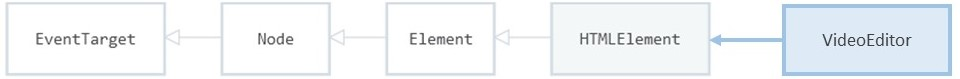
\includegraphics[width=1\textwidth]{images/inherit.jpg}
\caption{DOM Inheritance}
\label{fig:HTMLInheritance2}
\end{figure}

In this way a new \emph{"Autonomous Custom Element"} was created. As seen in the examples, these are elements that do not directly inherit from other elements in the HTML vocabulary (apart from the HTMLElement root). As a matter of fact, the API allows to create two types of custom elements. The second type is called \emph{“Customized built-in Element}”, meaning that the custom element extends a built-in HTML element. For example a HTML "p" tag, standing for a paragraph element or the HTML “img” tag standing for image element, and so on.
At the time of writing, the Customized built-in elements have a slightly more limited browser support\footfullcite{canIUseCustomElems}. Furthermore, in this work only Autonomous Custom Elements were used. 

Another important feature of Custom Elements are lifecycle hooks. These hooks – or more precisely, callback functions – can be defined in the class constructor and are automatically executed when elements enter one of the following states\footfullcite{googleWC}:

\begin{itemize}
\item connectedCallback: when the element is appended for the first time into a document’s DOM.
\item disconnectedCallback: when the element is removed from a document’s DOM.
\item adoptedCallback: when the element’s is moved to a new document.
\item attributeChangedCallback: when the element’s attributes are added, removed, or changed.
\end{itemize}

A frequent usage example can be made by considering Custom Element initialization and the update phase. The former triggers a connectedCallback method. Within this method, an initial state of the Component can be set: namely, API calls to populate the User Interface, registration of event handlers etc. Later an update phase can occur when one or more Component attributes change thanks to the attributeChangedCallback method. This is the case of reacting to user actions such as form actions, resolution changes, various interactions on interactive elements and so on. These changes can be automatically captured and reflected dynamically thanks to Component attributes. For example, if users interact with a server, the application state could change. A common scenario is generating a loading state. While the application is waiting for the server response, it can generate the appropriate feedback (a spinner element, helpful text messages etc.).

\subsection{Shadow DOM}
\label{subsec:shadowDOM}

Shadow DOM API as referred in the standard, can be defined as: 

\begin{displayquote}

“A set of JavaScript APIs for attaching an encapsulated "shadow DOM” tree to an element — which is rendered separately from the main DOM document — and controlling associated functionality.”\footfullcite{whatwgSD}

\end{displayquote}

In other words, it enables to attach a separate, encapsulated DOM which is isolated from the rest of the page. This is particularly useful for Custom Elements. It implies that the functionality defined inside a component, i.e., styles, markups and behaviour is limited (encapsulated) within the Shadow DOM boundaries. In other terms, anything happening inside a Shadow DOM does not have any effect outside of it.

The Shadow DOM API method, “attachShadow”\footfullcite{mdnShadow} is used for attaching a Shadow DOM to an HTML Element (therefore any\footnote{Shadow DOM cannot be attached to every HTML element, a list of HTML element supporting this functionality can be found in the documentation.} autonomous custom elements defined in the previous section).

The consequences can be seen with an example. Given two components: “Component A” and “Component B”, supposedly both containing an HTML input element with an attribute, “id” set to value “input-1”. Standing to the HTML best practices “ids” should be unique in the entire document. This is not the case of this example as “Component A” DOM is fully separated from “Component B” DOM. Therefore, elements referred by the id “input-1” can be styled and referenced separately for the two components even if they were instantiated inside the same application.

Code \ref{codeShadowDOM} shows the shadow DOM attachment to a standard HTML Element and a Custom Element.
\\
\begin{lstlisting}[caption={Shadow DOM attachment},label={codeShadowDOM}, language=JavaScript]
// Shadow Root attachment to HTML <article> element
const htmlInput = document.createElement("article")
        .attachShadow({ mode: "open" });

// Shadow Root attachment to Custom Element
class VideoEditor extends HTMLElement {
    constructor() {
        super();
        // Some element functionality here
        ...
        this.attachShadow({ mode: "close" });
    }
}
\end{lstlisting}

The Shadow DOM API allows to attach two types of Shadow DOM. An open shadow root allows accessing the DOM outside of the HTML element definition while a closed shadow root does not expose the DOM outside of the element. In the latter case the DOM cannot be referenced and accessed outside of its context. In theory, it exists in the flow of the document since it is rendered but its functionality is hidden from the rest of the page. However multiple ways of “hacking through” the limitations of closed shadow root exist\footfullcite{ShadowDomBlog}, therefore the usage of open shadow DOMs is recommended.

Finally, an overview to summarize the concepts introduced can be seen in Figure \ref{fig:shadowDom}: DOM Tree and Shadow Tree.

\begin{figure}[H]
\centering
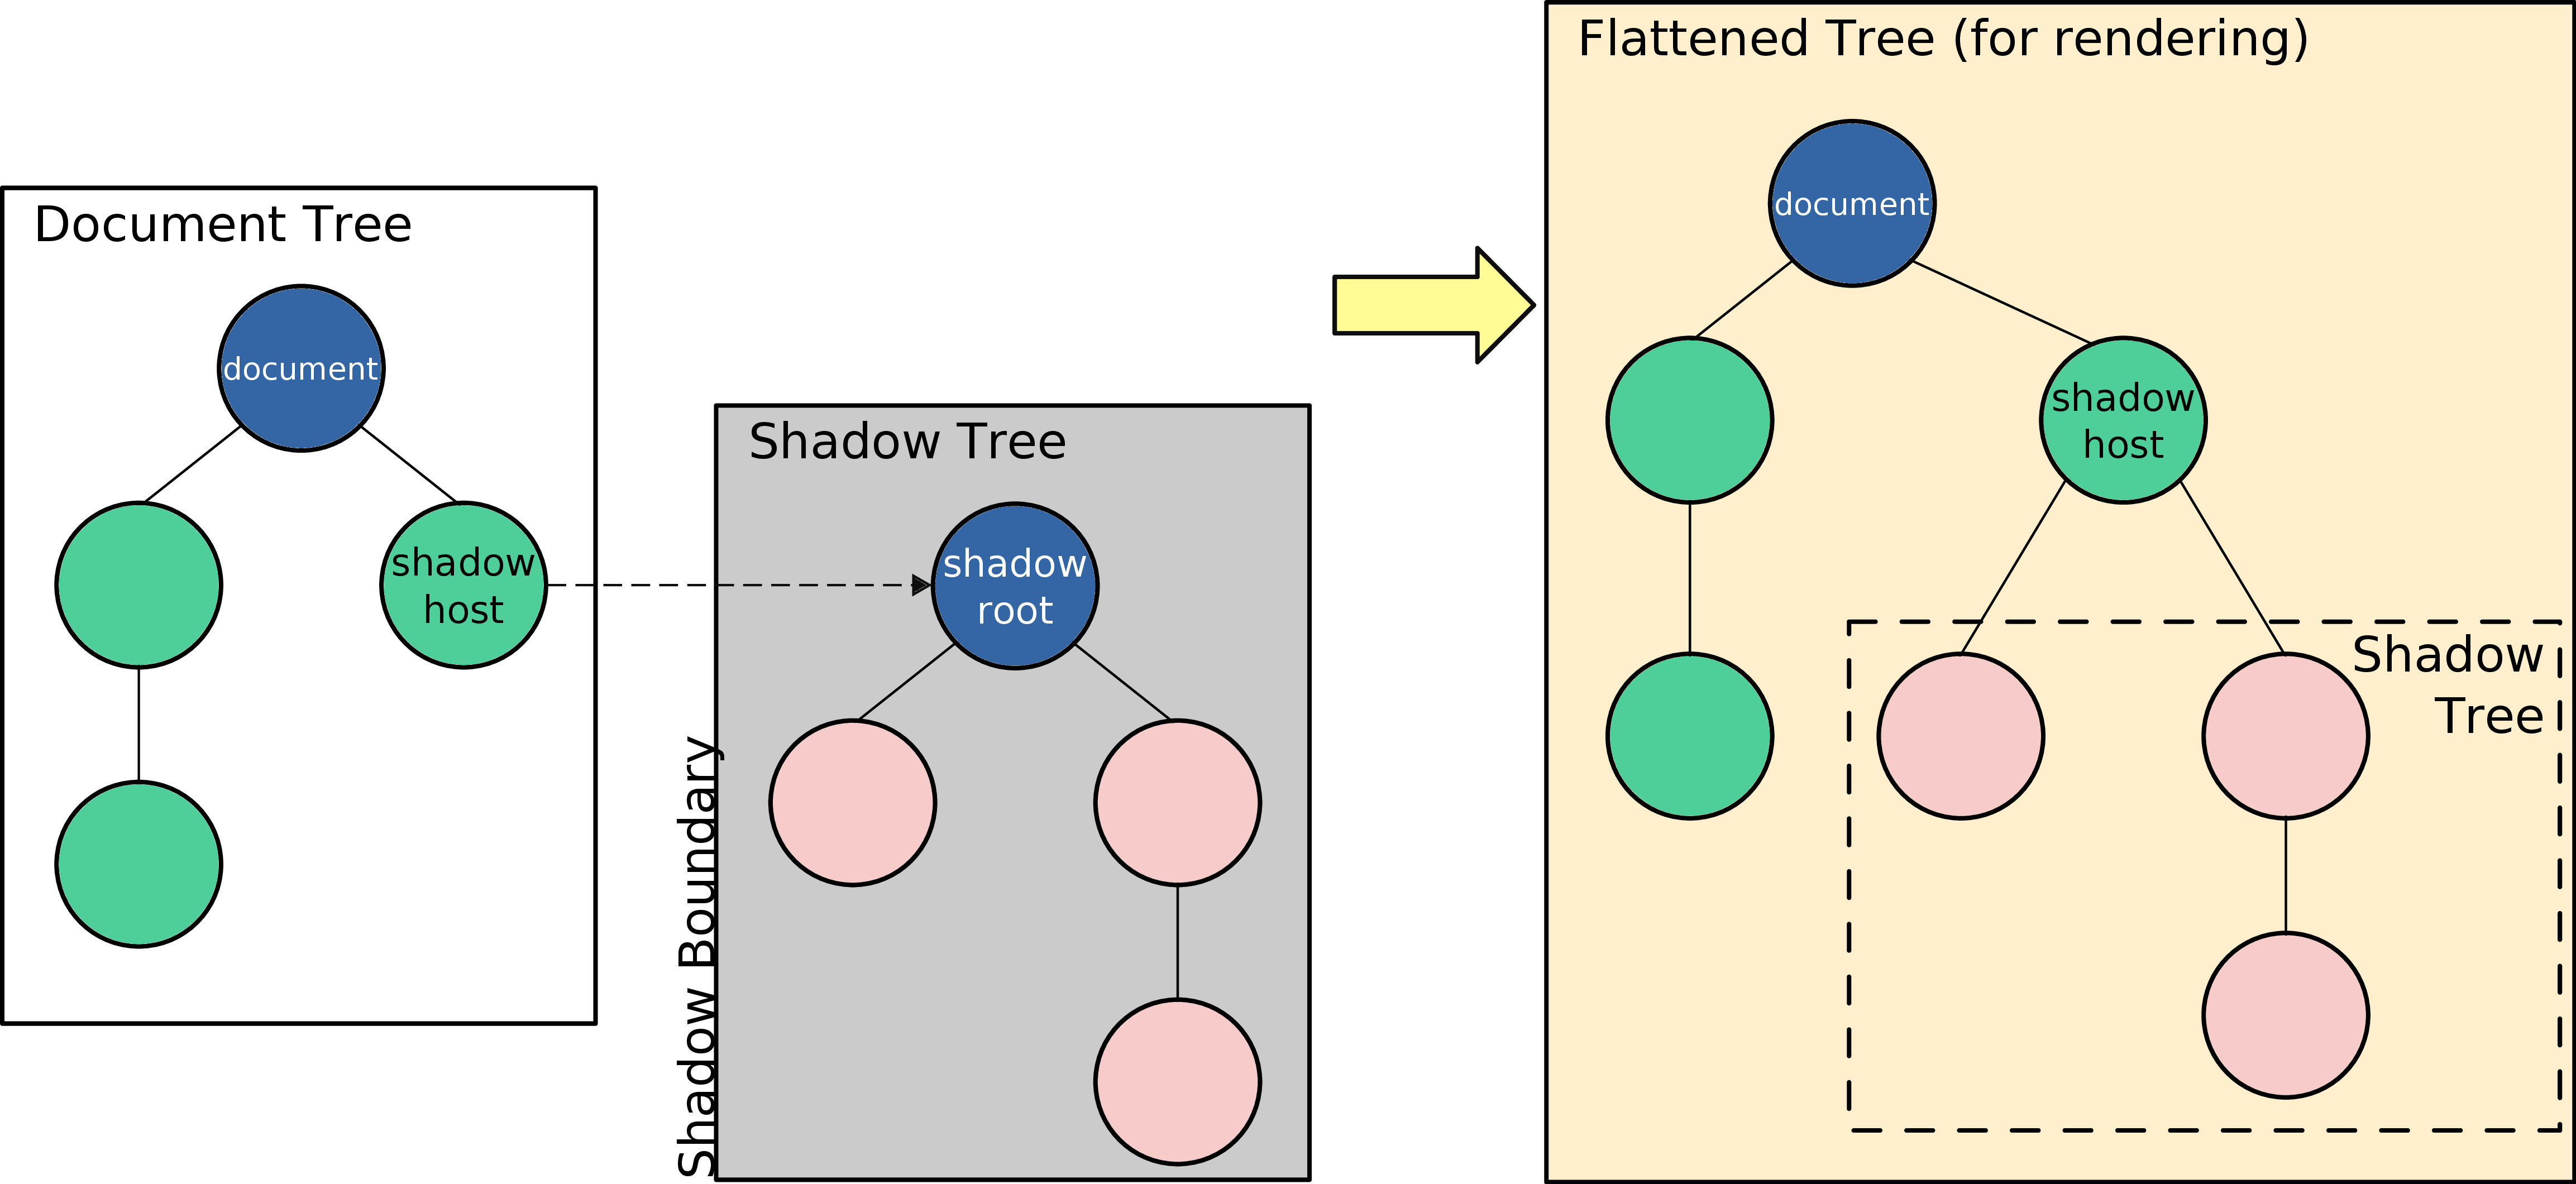
\includegraphics[width=1\textwidth]{images/shadowdom.jpg}
\caption{DOM Tree and Shadow Tree (from Mozilla Developers Network, licensed under CC-BY-SA 2.5)}
\label{fig:shadowDom}
\end{figure}

Some basic terminology is also explained in the documentation\footfullcite{mdnUsingShadow}:

\begin{itemize}
\item Shadow host: The regular DOM node that the shadow DOM is attached to.
\item Shadow tree: The DOM tree inside the shadow DOM.
\item Shadow root: The root node of the shadow tree.
\item Shadow boundary: the place where the shadow DOM ends, and the regular DOM begins.
\end{itemize}

\subsection{HTML Templates}
\label{subsec:HTMLTemplates}

The HTML Templates technology consists of HTML template\footfullcite{whatwgTemplate} and HTML slot\footfullcite{whatwSlot} elements, specified by the W3C living standards. Among the main characteristics, they allow to produce reusable content that can be defined, referenced by JavaScript, and later instantiated inside the DOM Document. This can be useful for creating content with redundant structure only once.

The Template element “is a mechanism for holding HTML that is not to be rendered immediately when a page is loaded but may be instantiated subsequently during runtime using JavaScript.”\footfullcite{mdnTemplate} This definition suggests that HTML structures of arbitrary complexity can be created and dynamically appended to the DOM Document.
\\
\begin{lstlisting}[caption={HTML Template creation},label={htmlTemplate}, language=HTML]
<template class="image-gallery">
    <ul class="gallery-list">
        <img src="firstImage.png" alt="first image description">
        <img src="secondImage.png" alt="second image description">
    </ul>
</template>
\end{lstlisting}

Notably, this approach can be used with and within Web Components to produce templates of components. Therefore, components can be put inside templates and instantiated when and where necessary.
While templates are a more general purpose mechanism, the slot element was introduced specifically for the Web Components technology context.  Thanks to the “slot” tag, developers can create placeholders inside Web Components that allow to instantiate additional children with their own separate DOM trees. Compared to templates, slots offer greater flexibility and configurability (intended as the possibility of instantiating dynamically generated markup). By expanding upon the last example, it should be possible to visualize how slots enable greater flexibility.
\\
\begin{lstlisting}[caption={Slotted templates},label={slottedTemplate}, language=HTML]
<template class="image-gallery">
    <ul class="gallery-list">
        <slot name="image-description"></slot>
        <img src="firstImage.png" alt="first image description">
        <slot name="image-footer"></slot>
        ...
    </ul>
</template>
\end{lstlisting}

From now on, any valid HTML element can replace the slot placeholders by referring to their name attribute (indeed, they can also be called “named slots”). A paragraph with an image description can be expected on top of the "img" element, also a footer containing the author’s credits and a hyperlink to other similar work can be imagined.

This procedure allows for greater reuse of specific parts of markup, the latter can be instantiated differently depending on the context. Another example comes from the work done for this dissertation project. The Query-Text Web Component – in practice a search bar – can be optionally instantiated with a “slottable” button coming from an external Web Components library with its own Shadow DOM and encapsulated behaviours (figures: \ref{fig:queryTextBase} Query-Text base class and \ref{fig:queryTextSlotted} Query-Text with slotted search button demonstrate these differences).

Overall, templates and slots in conjunction allow for a powerful composition of markup, thus preventing redundancy and shortening the code. 

\section{Web Components libraries}
\label{sec:wCLibraries}

Web Components libraries were created with the main intent of simplifying and speeding up the development process. Libraries usually provide some sort of abstractions on top of the native Web Components for efficiency and in order to enable new features.

During the planning phase, some of the most popular and active Web Components libraries were considered for adoption: LitElement\footfullcite{lit}, FAST\footfullcite{fast}, hybrids\footfullcite{hybrids}, Stencil\footfullcite{stencil} and Adobe Spectrum\footfullcite{spectrum}.
By looking at these proposals and the companies behind each library, it emerges that some important organisations are investing in and actually using the Web Components technology. Namely, FAST is authored by Microsoft, LitElement by Google, Adobe by Adobe, and Stencil is made by the Ionic Framework team\footfullcite{ionic}. Hybrids is an exception since it is a community based effort.

As anticipated, LitElement was the choice for the dissertation’s project. It originated from Google’s Polymer library. This library was mainly chosen due to its popularity, the presence of a large and thriving community involved in the project and a high quality exhaustive documentation\footfullcite{litDocs}. Certainly, the features offered and the fact that LitElement is fully compatible with all the browsers which adopt the native Web Components technology was also crucial during the decision making process.
Indeed, LitElement is an abstraction over the native HTMLElement. By using LitElement class-based components, developers are extending the LitElement class which in turn extends HTMLElement behind the scenes.

LitElement provides features like reactive state, scoped styles, and a declarative template system that are extensively used during this project’s development. The former can also be defined as reactive properties, i.e., properties that hold the state of the component. This implies that changing one or more of the components' reactive properties automatically triggers an update cycle, re-rendering the component. From the developer point of view this is a big simplifier. Indeed, by combining another LitElement feature, declarative templates, the User Interface can be efficiently updated and almost without writing any code.

Lit templates allow to render dynamic contents thanks to many helper operators. As stated in the official documentation\footfullcite{litTemplates}:

\begin{itemize}
\item Expressions: Templates include dynamic values called expressions that can be used to render attributes, text, properties, event handlers, and even other templates.
\item Conditionals: Expressions can render conditional content using standard JavaScript flow control.
\item Lists: Render lists by transforming data into arrays of templates using standard JavaScript looping and array techniques.
\end{itemize}

Finally, thanks to the scoped styles feature, LitElement automatically attaches a Shadow DOM to the component. This allows to define encapsulated styles that affect only the components context.

\section{Project idea and Front End Software Architecture}
\label{sec:SoftwareArchitecture}

In this section, a brief discussion about the project idea and its evolution will be introduced followed by a description of the adopted front-end software architecture. As mentioned in this work’s introduction, the application idea was originated from the activities related to the “PH-Remix” interdisciplinary project.

The practical project work of this dissertation is mainly concerned with the development of an in-browser multimedia editing tool. This tool – called “Remix environment” or “Remix platform” in the PH-Remix context – allows for discovery and reuse of multimedia content.

Two phases of development can be extrapolated from a temporal perspective. In the first phase, the application was subject to goals and requirements defined for the “PH-Remix” project. In the second phase, the application was expanded upon to fit a more general scenario. These two phases ought not to be considered as mutually exclusive. On the contrary, thanks to modularity and configurability, the application can accommodate the requirements of the “PH-Remix” project as well as alternative project ideas and implementations. The latter point might be viewed as particularly interesting in the context of this work’s narrative. By demonstrating that multiple applications can be made using the same components it seems that a remix can be applied to the software world. The components can be assembled like LEGO blocks alongside with other components developed from the community, an argument best exemplified in paragraph \ref{sec:appExamples} \emph{Examples of applications}.

The first step of this work involved defining an appropriate software architecture and was done thanks to the collaboration with the “PH-Remix” project members. Consequently, the project was initialized with the subsequent goal of producing an application prototype. The prototype can be seen as an evolutionary prototype\footfullcite{wikiPrototyping} due to the adopted architecture that can be easily refined and expanded.

The front-end architecture was driven by the principles of microservices architecture\footfullcite{redHat}. Namely, the Web Components technology is used as foundation for adopting the separation of concerns design principle\footfullcite{wikiSoc} between application components. The main choices for the adoption of Web Components adoption were made by keeping in mind the benefits of flexibility, maintainability, and scalability. Also, for the sake of efficiency and productivity LitElement was adopted as the Web Component library.

The core front-end structure is composed of the following components: 

\begin{itemize}
\item Video-Editor-App
    \begin{itemize}
        \item Video-Preview
        \item Track-Editor
    \end{itemize}
\item Query-Ui
    \begin{itemize}
        \item Query-Text
        \item Result-Media
    \end{itemize}
\end{itemize}

As seen in the list above, two components’ levels can be distinguished. On the top-level, the “Video-Editor-App” and “Query-Ui” act as wrappers. They can instantiate the components below. They are designed for managing the communication between the client side and the server side through API calls. Therefore, they are more project specific – than the components at one level below – and must be configured in order to request and retrieve application specific data. Similarly, the Query-Ui acts as wrapper enabling communication between Query-Text and Result-Media components.
This suggests another architectural choice. The rest of the components are isolated and are not concerned with the state of other components. Strictly, the communication with the external world is not allowed. They can be used independently in other application contexts and for different purposes. In other words, they should be operational and testable in isolation.
However, communication is possible, and necessary to compose the components into a coherent application. Therefore, the following planned communication rules were established. Data can be passed top-down through properties and can be lift-up through Custom Events\footfullcite{mdnCustomEv}. For example, Query-Ui receives a search string from the Query-Text component, sends it through an API to a search engine and returns the results to the media viewer, also known as “Media-Result”.

This architecture can be seen in Figure \ref{fig:appMockUp} Application architecture Mock-up.

\begin{figure}[H]
\centering
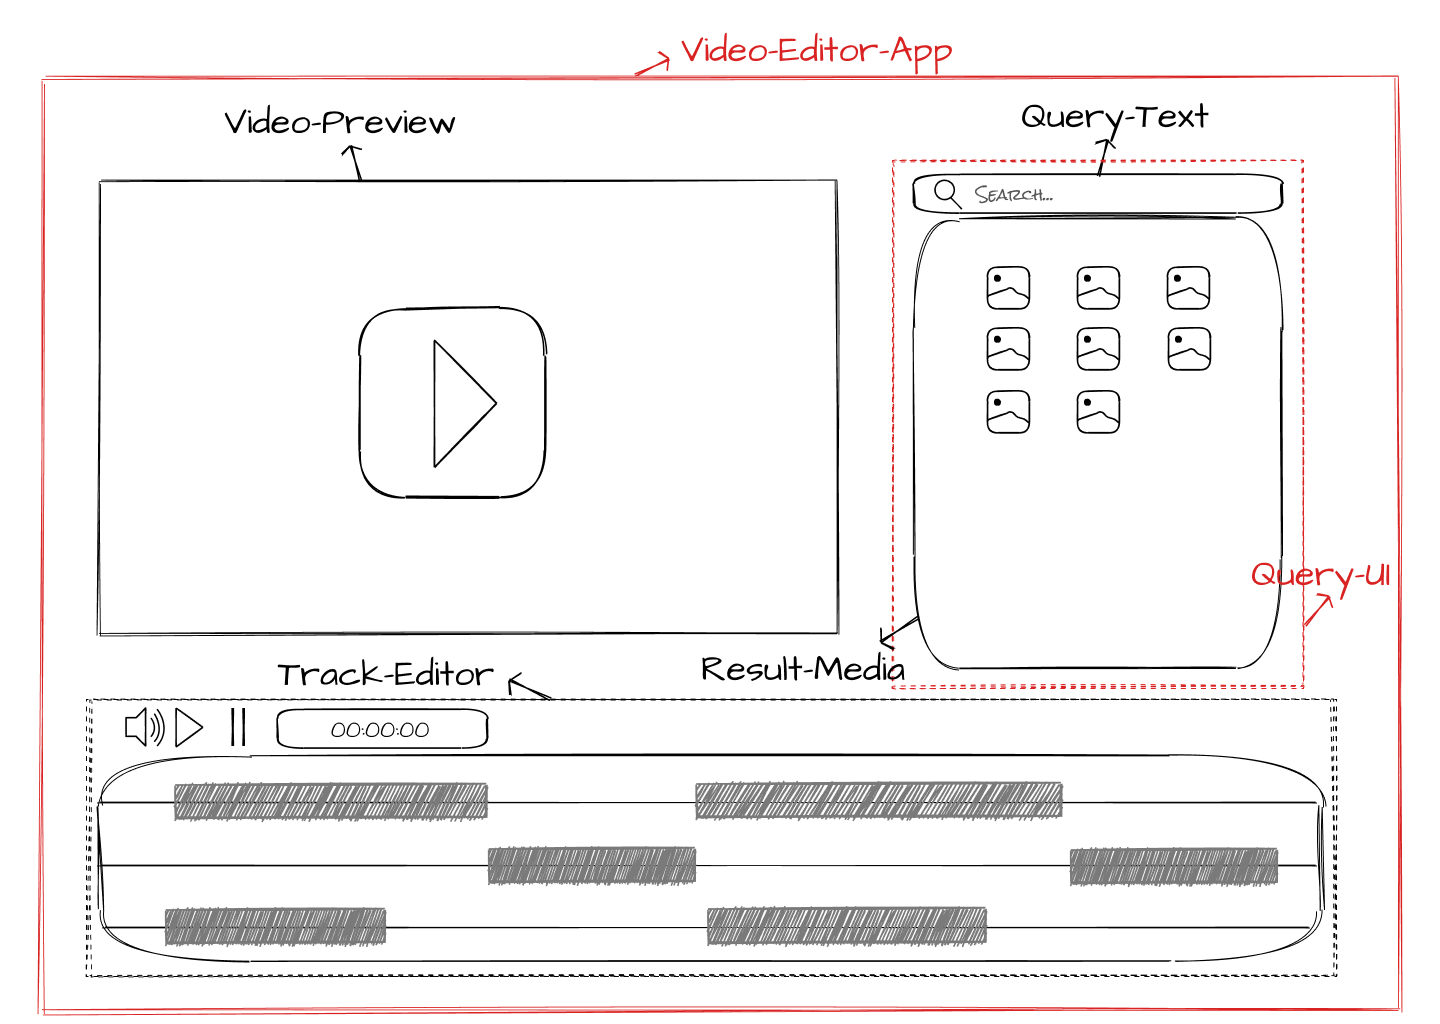
\includegraphics[width=1\textwidth]{images/Wireframe.png}
\caption{Application Mock-up}
\label{fig:appMockUp}
\end{figure}

Each of these components will be explained in more details in the next sections. 

Another important aspect regards the organizational choices. That is, the way the repository is organised, how the code structure is made, how the build and deploy phases are designed.

Firstly, components were designed to be independent and therefore, they can reside within separate online repositories. From a practical point of view, after some development iterations, an alternative approach was adopted. A monorepo\footfullcite{atlassian} setup was undertaken with the help of the Lerna\footfullcite{lerna} library. Monorepo is a repository which contains a number of projects inside the same centralized container. Since the components are used as dependencies which are injected or arranged into an application, this helps to organise and speed up the development. Nevertheless, nothing prevents from extracting components into separate repositories anytime.

\begin{figure}[H]
\centering
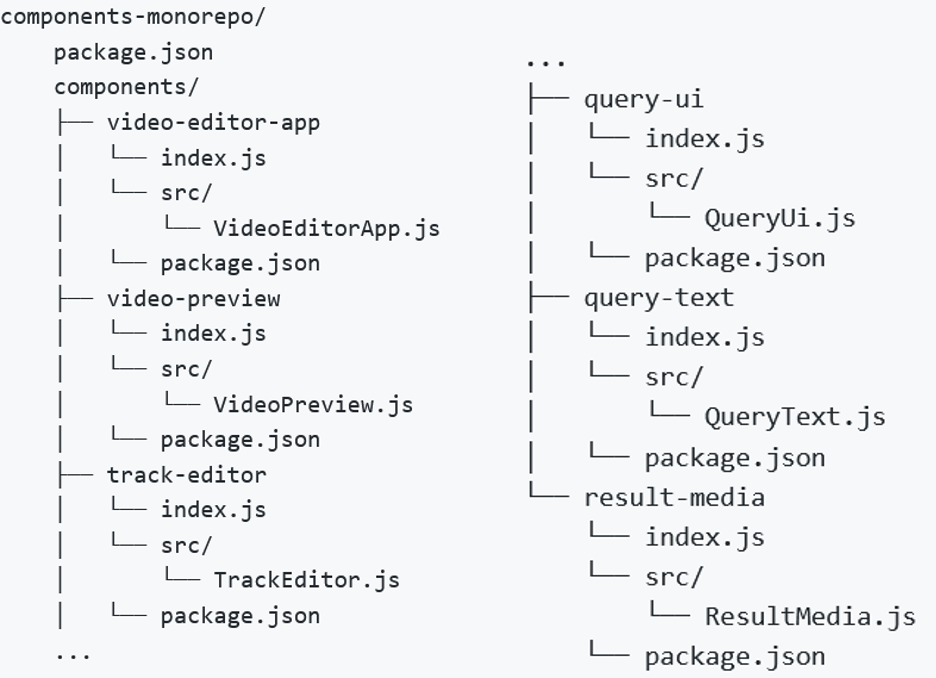
\includegraphics[width=0.8\textwidth]{images/repository.png}
\caption{Project repository structure}
\label{fig:repoStructure}
\end{figure}

The figure \ref{fig:repoStructure} shows a flat structure of components, although they can be dependent on one other. For example, “Query-Ui” can depend upon “Query-Text” specifying the latter as a project dependency inside its “package.json”. By adopting a monorepo structure the dependencies are always at hand, ready to be modified and at the same time they maintain their own commit history. Lerna is a tool that further optimizes this workflow. Among the most prominent features, it allows for dependency hoisting, versioning with the possibility of publishing components into registries like npm, and many others.

In addition, the repository structure is well suited for automation. In particular, the “index.js” file provides an entry point for every component. In this context JavaScript module bundlers can be easily implemented.
\\
\begin{lstlisting}[caption={Component entry point example},label={componentEntrypoint}, language=JavaScript]
import { QueryText } from "./src/QueryText.js";
window.customElements.define("query-text", QueryText);
\end{lstlisting}

The figure above depicts the Query-Text component although its structure is identical for every other component. Again, the objective is to offer a robust way of distributing the application as a whole and a future-proof structure for project evolution. Indeed, the last step of a development iteration in the software world is usually informally referred to by the colloquial expression “going to production”. The practical meaning is about publishing the code to the server and therefore offering it to the final users. At this point the common wish is to have the most optimized code possible. In the web development scenario this can be done with the help of module bundlers. Among prominent features, they allow to resolve dependencies, produce module maps for efficiency, and subsequently minify all the code.

Finally, several dependencies providing additional features are shared by all the components, therefore they will not be included in the descriptions contained in the next paragraphs. The dependencies were chosen and adopted following the Open Web Components initiative\footfullcite{openWC} indications. Their mission is to provide a list of best practices and recommendations for developing and sharing Web Components.

Therefore, a brief list of development dependencies is included in the project. Firstly, the purpose is indicated followed by a tool or a list of tools names and their brief description.

\begin{itemize}
\item Linting and Code checking: ESLint\footfullcite{esLint}, Prettier\footfullcite{prettier}. 
    \begin{itemize}
        \item These tools allow to keep consistent code formatting styles and avoid the most common problems by performing a statical code analysis.
    \end{itemize}
\item Testing: Karma\footfullcite{karma}, Mocha\footfullcite{mocha}.
    \begin{itemize}
        \item Testing environment for unit testing, integration testing and mocking.
    \end{itemize}
\item Interactive documentation: Storybook\footfullcite{storybook}
    \begin{itemize}
        \item It allows to visually describe the components with all the states they can assume.
    \end{itemize}
\item Building and deployment: Rollup\footfullcite{rollup}
    \begin{itemize}
        \item JavaScript module bundler used for library or application deployment.
    \end{itemize}
\end{itemize}

The next paragraphs introduce and briefly explain each component. The goal is to provide the core information about their structure and present some of the most interesting challenges encountered during development. Therefore, the next sections are not intended as a software documentation guiding through all the processes from installation to deployment. The documentation can be found by following each component’s links or by exploring the project’s root repository\footfullcite{rmxRepo}.

\section{Searching and displaying results}
\label{sec:searchingResults}

Searching and displaying the retrieved results can be considered pivotal for applications whose success can be largely measured in terms of the quantity and the quality of offered resources. Consequently, the main benefits that come from a good implementation might involve improved content discoverability and better user engagement.

These objectives were pursued by developing three components. First, a component called Query-Ui\footfullcite{rmxQueryUI} will be introduced. It is a connector between the client and server side and can be seen as a top level wrapper governing the functionalities below, of its children’s components. Indeed, it instantiates two components: “Query-Text”, which manages the search and autocomplete feature while “Result-Media” is concerned with the rendering of results found.
Notably, Query-Ui manages all the logic and information flow coming from the instantiated components. It also sends and receives data from external APIs, thereby passing data “downwards”, to the wrapped components.

An example of this relationship can be seen in the Code below.
\\
\begin{lstlisting}[caption={Query-Ui component instantiation},label={queryUi}, language=HTML5]
<query-ui>
  <query-text 
  .dictionaries=${this.dictionaries} placeholder=${this.placeholder}>
  </query-text>
  <result-media 
  .answerSet=${this.searchResults} headerTitle=${this.headerTitle}>
  </result-media>
</query-ui>
\end{lstlisting}

In this simplified example taken from one of the possible application configurations, properties and attributes are passed down to the components. Continuing with this practical example, Query-Ui internally makes an API call to the server side. In return, the endpoint responds with a dictionary – a list of words that can be autocompleted – which can be then passed to the search component. Namely, Query-Text. The principles guiding the de facto search feature are similar. The difference in implementation regards the presence of an event listener which is triggered every time users make a search. Ultimately, the results generated from the server are passed to the result viewer component, via the “answerSet” property, which renders them.

\subsection{Search component}
\label{subsec:searchComponents}

The Search component, named “Query-Text”\footfullcite{rmxQueryText} provides search and autocomplete functionalities within multi-keyed dictionaries of strings.

The idea behind Query-Text was to create a “google-like” search functionality based on lists of keywords. This is done by providing a list of prefixed dictionaries during the component instantiation. The component extracts keys from the dictionary and uses them as prefixes for autocompletion purposes. An example of valid dictionaries – not to be confused with dictionary data structures present in many programming languages – is exemplified the Code below.
\\
\begin{lstlisting}[caption={Dictionaries examples},label={dicts}, language=JavaScript, numbers=none]
{
    "filmmaker:":
        ["Martin Scorsese", "Ridley Scott", "Woody Allen", ...]
    "#:":
        ["goat", "chair", "mountain", ...]
    ...
}
\end{lstlisting}

In this example, two prefixes are present: “filmmaker:” and "\#". When users start typing one of the recognised prefixes, autocompletion based on that prefixed list of strings will be proposed. For example, by typing “\#:mou” a suggestion for the word “mountain” will be made.

Finally, by pressing the “ENTER” key or alternatively by clicking on the search button (if present), the component emits an event (through Custom Event bubble\footfullcite{mdnEvBubble}) with the actual value of the query string. An important feature is implemented to provide “fuzzy search” with autocompletion when user types into the search bar. Fuzzy search allows to tackle the possibility of typing errors made by users. A configurable options list is implemented with a scoring system offered by "Fuse.js" library\footfullcite{fuse}. Indeed, for example, if the word “montan” is typed, the user will be offered the “mountain” suggestion.

\begin{figure}[H]
\centering
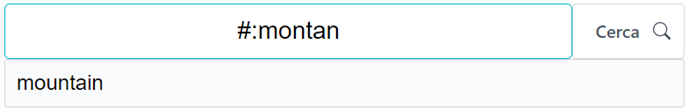
\includegraphics[width=0.8\textwidth]{images/autosuggest.png}
\caption{Query-Text autosuggestion feature}
\label{fig:queryTextAutosuggest}
\end{figure}

One of the possible issues that could arise regards the component performances. Especially when included within a more complex application, a performance-related issue emerges when users start to type fast onto the search bar. This implies the generation of a large number of DOM events and API calls if users decide to search the typed text. This issue was tackled by implementing a “debounce”\footfullcite{cssTricks} technique which limits the quantity of processed events. With configurable parameters, this instructs the autocomplete function to wait some arbitrary period of time in the order of milliseconds before taking any further action. Namely, it suggests words from the dictionary or sends the searched text to the search engine via API.

Finally, two examples of Query Text are exemplified in the figures below.

\begin{figure}[H]
\centering

\includegraphics[width=0.8\textwidth]{images/QueryText.png}
\caption{Query-Text base class}
\label{fig:queryTextBase}
\end{figure}

\begin{figure}[H]
\centering

\includegraphics[width=0.8\textwidth]{images/QueryTextSlotted.png}
\caption{Query-Text with slotted search button}
\label{fig:queryTextSlotted}
\end{figure}

The Figure \ref{fig:queryTextBase} shows the bare minimum component. Secondly, the figure \ref{fig:queryTextSlotted} shows an example of a button instantiated within the Query-Text slot.

\subsection{Results viewer component}
\label{subsec:resultsComponents}

As the name suggests, the “Media-Result” component renders some results onto the interface. For this project, search results are displayed as a gallery of thumbnails allowing for content selection and discovery. Importantly, the figures – or cards, as they are commonly called across UI libraries – can be dragged away from the component. This feature enables many possibilities as explored more in detail when introducing the track editor component. Specifically, with the help of the native Drag and Drop API\footfullcite{mdnDnD} some information about the object can be transferred through the drop event.

The adopted preview style can be seen in the Figure \ref{fig:mediaResults} Media-Result example.

\begin{figure}[H]
\centering
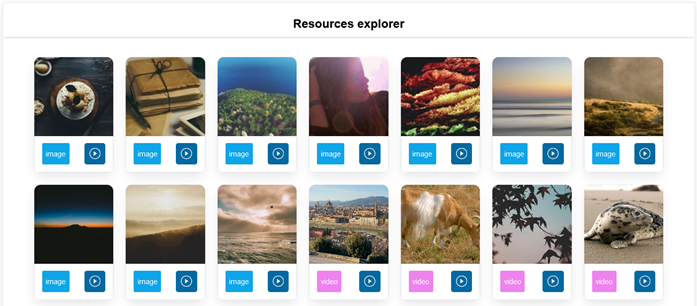
\includegraphics[width=1\textwidth]{images/ResultsMedia.png}
\caption{Media-Result example}
\label{fig:mediaResults}
\end{figure}

As mentioned before, these figures can be dragged and dropped to any valid drop target. Indeed, when users start dragging an object from the gallery,an event is triggered. This event is connected to the creation of a DataTransfer object\footfullcite{mdnDataTransf} containing all the necessary information to be transferred. For example, dragging a thumbnail that represents a video implies the insertion of the video duration onto the transferred data object. The latter can be read once the dragged item is dropped.

Additional features can also be optionally enabled. Since image thumbnails might not always be self-explanatory, the tooltip feature is also implemented in this project. Users can find further details about the resource by “hovering” on top of each media result. Continuing with the video result example, a tooltip may contain information about its title, duration, etc. Lastly, users might also be interested in reproducing the media directly inside the application. This is done by pressing the “play” button in combination with the “Video-Player” component which will be discussed in \ref{subsec:mediaPreview} Media Preview component.

\section{Multimedia Editor}
\label{sec:multimediaEditor}

The most characterizing piece of this project is the Multimedia Editor. It is a top level wrapper that orchestrates the application specific behaviour. The Multimedia Editor is called “Video-Editor-App” in the project repository but by design it should be re-named and configured in relation to the application purpose. In this case, it instantiates the Track-Editor and the Video-Preview components.

As a result, the application allows to combine and arrange image, sound, and video resources by dragging them from the Result-Media component into an interactive track. Subsequently, the elements arranged in the track can be viewed inside a player and potentially exported with the help of a back end infrastructure. Although combine and preview operations are the concern of the respective components, the Multimedia Editor has a key role in making them work together. Similarly to Query-Ui, it can communicate with the outside world through APIs.

The following markup reflects the relationship between components.
\\
\begin{lstlisting}[caption={Video-Editor-App component instantiation},label={videoAppComp}, language=HTML5]
<video-editor-app>      
      <video-preview
        .resources=${this.resources}
        .singleMediaPreview=${this.singleMediaPreview}
        .executeSegmentsPreview=${this.playSegments}
        .terminateSegmentsPreview=${this.endSegments}
      ></video-preview>
      <query-ui></query-ui>
      <track-editor
        draggedElementType=${this.draggedElementType}
      ></track-editor>
</video-editor-app>
\end{lstlisting}

The figure shows some of the properties that are used for synchronising the Track-Editor with its preview. As a matter of fact, the Video-Editor-App also manages the data flow originated from the Track-Editor. This cannot be seen in the markup because of the already mentioned design decision: “data can be passed top-down through properties and can be lift-up through Custom Events”. The latter explains the logic behind the interaction. This can be further demonstrated with the help of a practical example.

A frequent scenario involves users that compose multimedia resources inside the editing track by dropping them from the content library of choice. At any moment it is possible to reproduce the arrangements made within Track-Editor component. At this point, the latter component sends an event upwards. This event is composed of a list of media elements – alongside information about their start and end dates – that were present inside the track at the exact time the “play” button was pressed. This information is captured by the Video-Editor-App whose job is to request media from external APIs. Lastly, when a successful response is available, the data is passed through to the Video-Preview, ready to be played. This behaviour will be discussed in further detail in the next sections.

\subsection{Track Editor component}
\label{subsec:trackEditpr}

“Track-Editor”\footfullcite{rmxTrackEdtior} is the most complex component created for this project application. It offers the core feature of arranging media content similarly to the way it is implemented by some of the alternative software for video-editing. Its peculiarity is that it offers this functionality directly from the browser level.

In detail, Track Editor can be composed of multiple tracks. Depending on the configuration, an arbitrary number of tracks can be used. Tracks refer to specific media types, for example: an audio, video, and image track. Every track has a temporal dimension which allows to perform some basic operations that are key for any editing tool. Indeed, a temporal marker is also implemented for keeping track of the currently reproduced media. This can be seen in the example below:

\begin{figure}[H]
\centering
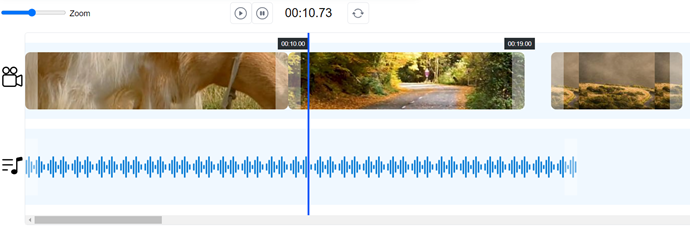
\includegraphics[width=1\textwidth]{images/TrackEditor.png}
\caption{Track Editor example}
\label{fig:trackEditor}
\end{figure}

Currently, the Track-Editor also allows to:

\begin{itemize}
\item Receive dragged media from the application library.
\item Arrange media elements inside the tracks by dragging them back and forth.
\item Resize or trim media in relation to their type.
\item Dynamically zoom in and out the track and re-dimension all the content inside of it.
\item Check whether a specific track can contain the dragged media type.
\item Play, pause, and reset the media reproduction.
\item Open a context menu for removing undesired media.
\end{itemize}

Some interesting points can be made from this list. First of all, operating with a content length of a few seconds is different from content whose duration might be in order of several minutes. This potential problem is mitigated by the zooming functionality. Also, some basic form of error prevention has been made to preserve the preview functionality. This is done by generating an informative message on the UI stating that a specific media type cannot be put inside a track.

Finally, the ability of playing, stopping, and resetting the current tracks state is synchronized with the temporal marker – namely, the blue line in \ref{fig:trackEditor} Track Editor example.

From the implementation perspective, when users press play, a Custom Event is dispatched. This event can be captured thanks to its bubble property, as showed in the Code below. 
\\
\begin{lstlisting}[caption={Track Editor event dispatch},label={customEvent}, language=JavaScript]
function dispatchEventForPreview() {
    const event = new CustomEvent('track-elements', {
      detail: {
        trackElements: this.segmentsOnTracks,
      },
      bubbles: true,
      composed: true,
    });
    this.dispatchEvent(event);
  }
\end{lstlisting}

This event transfers the current state of the Track-Editor. At a later stage this event can be captured and used for generating API requests.

\subsection{Media Preview component}
\label{subsec:mediaPreview}

The final part of this application is the media preview. The component that manages the preview is called “Video-Preview”\footfullcite{rmxVideoPreview}. As discussed in the previous paragraph, its main purpose consists in reproducing a synchronised preview of the media from the Track-Editor. Generally speaking, it can preview any number of media content, starting from a single preview to a large number of media with different media types.

An interesting implementation choice can be derived from the synchronization feature. It might be argued that the component has intuitively some sort of an internal clock or at least some way of keeping track of the elapsed time. As a matter of fact, in this case this is not entirely true. Contrary to the Track-Editor, which implements an internal timer that guides the component state. It turns out that “Video-Preview” does not necessarily need one. And yet it works. Walking through an example may effectively demonstrate how things work internally. Before jumping into the example, a possible way of instantiating the component is presented in the figure below.

An interesting implementation choice can be derived from the synchronization feature. It might be argued that the component has intuitively some sort of an internal clock or at least some way of keeping track of the elapsed time. As a matter of fact, in this case this is not entirely true. Contrary to the Track-Editor, which implements an internal timer that guides the component state. It turns out that “Video-Preview” does not necessarily need one. And yet it works. Walking through an example may effectively demonstrate how things work internally. Before jumping into the example, a possible way of instantiating the component is presented in the Code below.
\\
\begin{lstlisting}[caption={Video-Preview component instantiation},label={videoPreview}, language=HTML5]
<video-preview
        ?displayLoadingScreen=${this.displayLoadingScreen} 
        ?stopPlayer=${this.stopPlayer}
        ?resumePlayer=${this.resumePlayer}
        .resources=${this.resources}
        .executeSegmentsPreview=${this.playSegments} 
        .terminateSegmentsPreview=${this.endSegments}
></video-preview>
\end{lstlisting}

In particular, the “resources” property contains all the media items to be previewed. Hence, a video would be inserted into a HTML video source tag, an image would reside within an HTML img source and so on.

Assuming the scenario of Track-Editor interaction with Video Preview. After putting an arbitrary number of media elements inside the tracks, the user presses the “play” button. Subsequently the following steps occur:

\begin{enumerate}
  \item All the media references are sent through a Custom Event.
  \item The Event is captured by the top level Video-Editor-App component. It requests all the items using API calls.
  \item The responses arrive asynchronously and are sent to the Video-Preview component for preview.
  \item Track Editor starts its internal timer and checks if at the time 00:00:00 (in the minutes/seconds/milliseconds format) any media element has been positioned into the track. If yes, the next step is executed, otherwise the timer runs until it encounters an element on the track.
  \item Track Editor emits the “executeSegmentsPreview” event containing one or more references to media elements that must be previewed.
  \item The Event is captured by the top level Video-Editor-App component and passed immediately to the Video Preview component.
  \item Video Preview selects the right resource(s) – from the resource list received in the step 3 – and starts the preview.
  \item Once the media element duration ends, the Track Editor sends a “terminateSegmentsPreview” event.
  \item The Event is captured by the top level Video-Editor-App component and passed immediately to the Video Preview component.
  \item Video Preview selects the right resource(s) – from the resource list received in the step 3 – and stops the preview.
\end{enumerate}

This workflow – apart from the asynchronous API operations – happens with a near real time precision and continues as long as the user does not stop the reproduction or there are no more elements to be played on tracks.

As exemplified, the above mechanism makes the whole synchronized preview system work without the necessity of implementing additional timers. The Track-Editor governs the current items being played. By adopting this implementation, the Video-Preview component is simpler and more performant.

\section{Application examples}
\label{sec:appExamples}

The main application example is a prototype made for the PH-Remix project. This application uses resources currently protected by copyright which belong to the Mediateca Toscana. At the time of writing, they are mainly documentaries. In this case the resources are short videos extracted from the original works. This is done by Artificial Intelligence algorithms as explained in this dissertation’s introduction. Figure \ref{fig:phRmxOverview} shows the application interface which reflects the components architecture as determined in section \ref{sec:SoftwareArchitecture} \emph{Project idea and Front End Software Architecture}.

\begin{figure}[H]
\centering
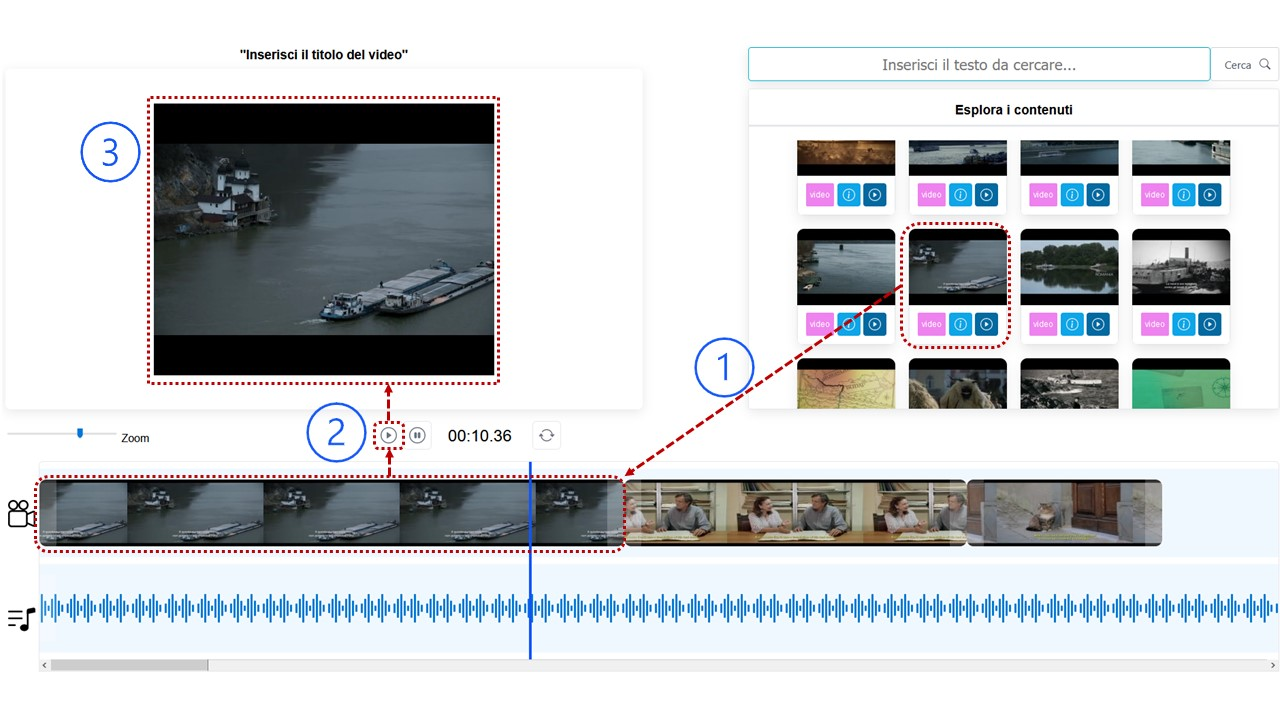
\includegraphics[width=1\textwidth]{images/PH-REmixannotatedUI.jpg}
\caption{PH-Remix annotated User Interface}
\label{fig:phRmxOverview}
\end{figure}

Firstly, four components can be seen directly in this example. The search bar or Query-Text component is positioned in the top-right corner. Then the middle-right side shows the content library. It can be explored thanks to the thumbnails, that is representative images extracted from each video clip. This is the part managed by the Result-Media component. At the bottom there is a track editor with two different types of media tracks. A video track on top and an audio track on the bottom. This part is managed by the Track-Editor component and it allows for positioning and arranging the media from the content library. Finally, on the top-left side a preview of the content can be reproduced. The Video-Preview component is used for displaying the elements from the editing track, as well as single video clips directly from the content library.

The Figure \ref{fig:phRmxOverview} has also been annotated to show some common actions that were explained earlier in this section. There are three steps necessary to select, insert and preview the content from the library. Step 1 consists in selecting the video clip to be arranged or edited inside the track. This is done by dragging the thumbnail directly into the corresponding media track. In this case a video clip is dragged to the video track. As seen in the interface, the latter proportionally expands the thumbnail length horizontally according to the duration of the video clip. This action can be repeated for every resource in the library. Subsequently, step 2 triggers the preview of the content that was positioned on the track. This happens by pressing the “play” button above the Track-Editor. Finally, step 3 allows to preview the sequence of the arranged content. This is the most common scenario for multimedia editing and can be repeated until the desired solution is reached.

Consequently, a more fine-grained look at the interface is shown by the figure below.

\begin{figure}[H]
\centering
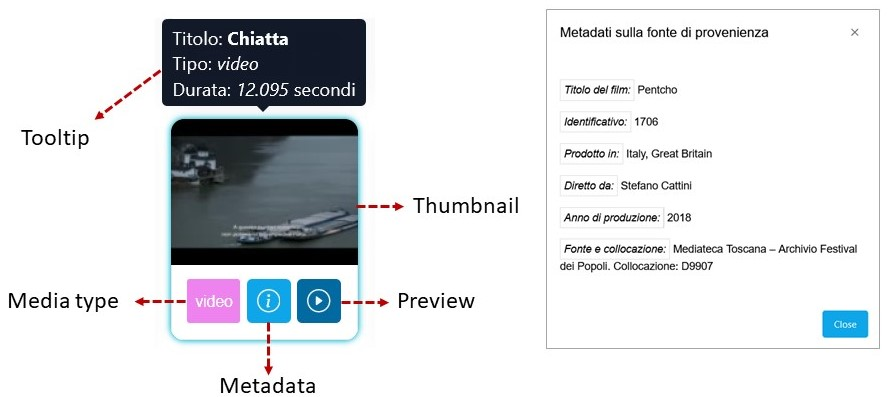
\includegraphics[width=0.8\textwidth]{images/phrDetails.jpg}
\caption{PH-Remix: Single resource entry (on the left) and modal window with details about the resource (on the right)}
\label{fig:phRmxDetails}
\end{figure}

This shows an annotated example (from the Italian version) of a single resource entry. The left-hand side displays the element state while the cursor is "hovering" over it. When users place their cursor on top of a library element, a tooltip with some basic information appears to disambiguate the nature of the resource. In this case the thumbnail seems to depict some sort of a barge floating on water. Indeed, the tooltip describes it as a “Barge” (“Chiatta” in Italian) alongside with the media type (video) and its duration in seconds. Below the thumbnail three elements of the interface allows to perform some actions with the element. These are always visible independently from the item’s state (like the aforementioned positioning of the cursor on top of it). Going from left to right, the media type is also specified within a coloured box, with a different colour for each media type. Then in the centre some more information about the object can be shown as exemplified on the right side of Figure \ref{fig:phRmxDetails}. This is particularly useful for content with cultural value. Indeed, in this case some metadata about the extracted clip and its original source are shown. For instance, the image displays the name of the documentary, its director, year of production, physical location, etc.

The last button allows to directly preview the video clip inside the Video-Preview component. This is useful to evaluate whether the visual content of the selected items is relevant for the editing action. Then it can be dragged to the track editor, as explained above.

On the other hand, the second example is a general-purpose application which integrates the resource from the Pexels API. Although at the time of writing the User Interface is almost exactly similar to the one of the PH-Remix, its peculiarity is that – thanks to the permissive license of the Pexels platform – it allows for legal remixing of content by everyone.
As a matter of fact, this consents unconstrained browsing of a rich Open Source catalogue of content. In particular, it consists of thousands of videos and images that can be freely built upon. Apart from the nature of the content itself, some features that are present in the PH-Remix example are not present in the general-purpose application and vice versa. For instance the ability of viewing object metadata is relevant to cultural heritage objects, but it may not be necessary for simple pictures made for fun.  


\clearpage

\addcontentsline{toc}{chapter}{Conclusions}
\chapter*{Conclusions}
\label{ch:conclusions}

lorem ipsum.

\printbibliography

\end{document}